\documentclass[a4paper,11pt]{kth-mag}
\usepackage{textcomp}
\usepackage[table]{xcolor}
\usepackage[hidelinks]{hyperref}
\usepackage{todonotes}
\usepackage{lmodern}
\usepackage{amsmath}
\usepackage{amsthm}
\usepackage[swedish,english]{babel}
\usepackage{modifications}
\usepackage{multirow}
\usepackage{textcomp}
\usepackage{listings}
\usepackage{color}
\usepackage{amssymb}
\usepackage{dirtree}
\usepackage{array}
\usepackage{pdfpages}
\usepackage{longtable}
\usepackage{siunitx}
\usepackage{nameref}
\usepackage{url}
\usepackage{xcolor}
\usepackage{comment}
\usepackage{graphicx}
\usepackage{float}
\usepackage[square,sort,comma,numbers]{natbib}
\usepackage{amsmath, amssymb}
\usepackage{changepage}
\usepackage{mleftright}
\usepackage{mathtools}
\usepackage[utf8]{inputenc}
\usepackage[T1]{fontenc}
\usepackage{enumitem}
\usepackage{algorithm}
\usepackage[]{algpseudocode}
\usepackage{mwe}
\hbadness=99999
% For nomenclature
\usepackage{etoolbox}
\usepackage{nomencl}
\usepackage{caption}
\usepackage{subfig}
\makenomenclature
% For pseudo algorithm code
\makeatletter
\def\BState{\State\hskip-\ALG@thistlm}
\makeatother
 

\extrafloats{1000}


\title{Comparison Between a Model Based and Data Based Controller Approach for a Mobile Sink in a Wireless Sensor Network}

\subtitle{Thesis WIP}
\foreigntitle{Title in Swedish goes here}

\author{Axel Karlsson \\ Bohan Zhou}
\date{\today}
\blurb{Master's Thesis at ITM\\Supervisor: Tong Liu \\ Examiner: Dejiu Chen}
\trita{TRITA xxx yyyy-nn}


\begin{document}
\frontmatter
\pagestyle{empty}
%\removepagenumbers
\maketitle
\selectlanguage{english}


\clearpage
\begin{abstract}
\noindent As smart cities are expanding, more and more problems concerning the energy consumption for Wireless Sensor Networks (WSNs) are arisen. In this work a WSN is defined as a two dimensional area which contains sensor nodes and a mobile sink, i.e. a movable base station. Since the area of such a network could be large and contain many nodes, it is of interest to compare two new energy methods within two different fields. \newline

\noindent This thesis work investigated a new method to cluster wireless sensor nodes together with two new control approaches for a mobile sink. In an WSN environment developed by the authors, a model based controller and a data driven controller for controlling a mobile sink was designed and deployed. By controlling the placement of the sink and the packet rate of all nodes the controllers were able to reduce the energy consumption of the entire system. \newline

\noindent The clustering method and two control approaches were compared on the metrics of energy consumed, data packets sent and the amount of data that can be sent with an energy unit. From tests conducted on the system the results show \dots \newline   


\noindent \textcolor{red}{TODO: Update with results and short discussion. Potentially write a short introduction to what a WSN is.}\newline

\noindent \textit{Keywords: Wireless sensor network, internet of things, nodes, mobile sink, base station, data packets, embedded systems, energy management, clustering, LEACH, cluster head, model based controller, MPC, optimization, data driven control, reinforcement learning, DQN, neural networks}
\end{abstract}
\clearpage
\begin{foreignabstract}{swedish}

Abstract in Swedish goes here. \newline


\noindent \textit{Nyckelord: Trådlösa sensor nätverk, internet of things, noder, mobile sink, basstation, data paket, inbyggda system, energihushållning, klustring, LEACH, klusterhuvud, modell baserad regulator, MPC, optimering, datadriven regulator, reinforcement learning, DQN, neurala nätverk}



\end{foreignabstract}
\clearpage

\chapter*{Acknowledgements}

\noindent We would like to thank the Mechatronics Department at KTH and especially our supervisor Tong Liu for the support provided during the thesis work. We truly appreciated your knowledge and contribution towards completing the thesis. A large gratitude goes to our examiner Dejiu Chen for helping us answer the research question and our thesis coordinator Fredrik Asplund for guiding us to the field of research. We would also like to thank Cybercom and our industrial supervisor Karl Hansen for fruitful discussions and supervision throughout the project. \newline
\newline 
\noindent Thanks also to John Hedengren from Brigham Young University for providing continous support for the GEKKO optimization suite. \newline
\newline   
\noindent Finally thanks to our colleagues, friends and family for being there when it mattered the most. 

    
\begin{flushright}
   Axel Karlsson \& Bohan Zhou \\
   Stockholm, July 2019   
\end{flushright} 

    

\clearpage
\tableofcontents*
\clearpage
\listoffigures*
\clearpage
\listoftables*

\makenomenclature
\renewcommand\nomgroup[1]{
  \item[\bfseries
  \ifstrequal{#1}{T}{Terminology}{\ifstrequal{#1}{S}{Symbols}{\ifstrequal{#1}{A}{Abbreviation}}}]}


\setlength{\nomlabelwidth}{5cm}
% Terminology
\nomenclature[T]{Cycle}{Sequence of transmission rounds before the LEACH protocol resets.}
\nomenclature[T]{Episode}{One run of the WSN environment from creating the WSN environment until all node are dead}
\nomenclature[T]{Reward}{Given to the agent in RL to promote desired behaviour}

% Abbreviations
\nomenclature[A]{$WSN$}{Wireless sensor network}
\nomenclature[A]{$CH$}{Cluster head}
\nomenclature[A]{$MPC$}{Model predictive control}
\nomenclature[A]{$NMPC$}{Nonlinear model predictive control}
\nomenclature[A]{$RL$}{Reinforcement learning}
\nomenclature[A]{$LEACH$}{Low-energy adaptive clustering hierarchy}
\nomenclature[A]{$BLEACH$}{Broadened LEACH}
\nomenclature[A]{$SoC$}{State of charge}
\nomenclature[A]{$MIL$}{Model in loop}
\nomenclature[A]{$NN$}{Neural network}
\nomenclature[A]{$DQN$}{Deep Q-network}
\nomenclature[A]{$MAE$}{Mean absolute error}
\nomenclature[A]{$CHS$}{Cluster head status}
\nomenclature[A]{$EC$}{Energy consumed}
\nomenclature[A]{$PR$}{Packet rate}
\nomenclature[A]{$ULC$}{Upper layer control}
\nomenclature[A]{$LLC$}{Lower layer control}
\nomenclature[A]{$API$}{Application Programming Interface}




% Symbols
\nomenclature[S]{$\alpha$}{Learning Rate}
\nomenclature[S]{$\epsilon$}{Exploration rate}
\nomenclature[S]{$\gamma$}{Learning rate}
\nomenclature[S]{$n$}{Current transmission round}
\nomenclature[S]{$P$}{Percentual CH distribution for LEACH}
\nomenclature[S]{$T$}{LEACH/BLEACH value function}
\nomenclature[S]{$E_{Tx}$}{Energy transmitted by a node during a time segment}
\nomenclature[S]{$E_{Rx}$}{Energy received by a node during a time segment}
\nomenclature[S]{$E_{gen}$}{Energy generated by a node during a time segment}
\nomenclature[S]{$J$}{Objective function}
\nomenclature[S]{$J*$}{Optimal value of objective function}
\nomenclature[S]{$K$}{Discrete step horizon length}
\nomenclature[S]{$\mathcal{R}$}{Reward set}
\nomenclature[S]{$\mathcal{A}$}{Action set}
\nomenclature[S]{$\textbf{x}$}{State vector}
\nomenclature[S]{$\textbf{u}$}{Control vector}
\nomenclature[S]{$PPJ$}{Packets per joule}
\nomenclature[S]{$PA$}{Packet amount}


\printnomenclature
\mainmatter
\pagestyle{newchap}

\chapter{Introduction}
\textit{This chapter will give an introduction into the field of Wireless Sensor Networks (WSNs) as well as the preliminary works that have been conducted in the field of study. The ethical considerations, the project outline, the problem statement and the research questions are also presented.}

\section{Background}

\noindent A hot topic in this day and age is the realization of the so called "Smart City", where wireless sensor networks (WSNs) are deployed in great amounts to monitor our living environments. The goal with these WSNs is to functionally and structurally improve the city’s sustainability and efficiency \cite{liu2017rf}. Since WSNs often contain many nodes, powering them on a large scale through the city power line or by batteries is not a feasible solution \cite{ruan2017energy}, \cite{ImportanceMitcheson2008energy}. Therefore, a general solution is to charge the nodes by self harvested energy. Due to that the self harvested energy is often inadequate, it is of great importance to achieve an efficient management on energy usage by proper clustering and control methods.\newline

\noindent A common strategy for energy management  is continuously relocating the network's receiving base station in order to accommodate to the varying level, generation, and consumption, of energy among the nodes \cite{torghabeh2010mobile}, \cite{heinzelman2000energy}. With regards to this, this thesis work presents the development, design and comparison of two optimal control designs, one data driven and one model based. Both regulate the position of the base station as well as the packet rates (PRs) of the station's connected nodes. The objective of this regulation is to maximize the amount of total data aggregated in relation to the total energy available. In addition to this a novel clustering algorithm is also devised. The research is conducted in collaboration with Cybercom Group AB.

\section{Earlier Works}
\label{ss:EarlierWorks}
\noindent The following works explores different aspects of the solution space. 

\begin{enumerate}
    \item In the year 2000, \textit{Wendi Rabiner Heinzelman et al.} proposed a new method for clustering wireless sensor nodes. The clustering method that was presented in this paper is called Low-Energy Adaptive Clustering Hierarchy (LEACH) and is based on electing sensor nodes as cluster heads (CHs) in a stochastic fashion. The role of a CH is to relay the data of its connected sub-nodes to the sink. After the CHs have been elected, the non-CH nodes connect to the CH that is closest to itself and the regular nodes communicate with the base station via the CH. It was shown that this clustering method improved the energy dissipation with a factor of 8. However, the LEACH clustering method does not take the state of charge (SoC) of the node into consideration when the CHs are elected \cite{heinzelman2000energy}.

    \item In 2010, \textit{Nasrin Abazari Torghabeh et al.} proposed a relocating system for a mobile sink that took the SoC, the number of connected nodes and distance to the sink of each CH as inputs. The authors accomplished this by implementing a controller for the sink movement that deployed fuzzy logic to assign varying degrees of "critical statuses" to each CH based on the aforementioned inputs. The results showed an increase in network life time, energy of network and alive sensors in relation to network round \cite{torghabeh2010mobile}.
    
    \item In 2011, \textit{Xue Jun Li et al.} released an article about possible applications of model predictive control (MPC) in WSNs. It discussed several methods that MPC can be applied to improve network capacity. It was concluded that MPC is a promising candidate for solving optimization problems in WSN systems such as power control \cite{li2011application}.
 
    \item In 2018, \textit{Fayçal Ait Aoudia et al.} proposed a novel energy management algorithm based on reinforcement learning (RLMan) which was deployed on every node in the wireless sensor node network to control its packet rate depending on current SoC. Unlike it's forerunners it only takes the current state of energy into account and not the current energy harvesting status. This allows the sensors to save energy which would otherwise go into the overhead accompanied with harvesting sampling. The method proved to be more efficient, with regards to network lifetime in relation to average packet rate, than all other methods tested against it \cite{RLbasedEHWSN_RLMAN}.
\end{enumerate} 

\noindent All the aforementioned works achieved promising results. However, the positioning of the sink with regards to its surrounding nodes as well as the PR of designated nodes are seldom controlled simultaneously. By implementing a controller capable of regulating both presents an opportunity for improved energy and data management.


\section{Project Outline}
\label{sec:prjoutline} 
\noindent In order to regulate the LEACH based WSN with respect to aforementioned variables, model based design strategy is employed to develop an optimal controller. Meanwhile, another strategy independent of the explicit dynamic models is also attempted to design a data-driven controller. While encountering the energy and data management optimization problem in this project, the aim is to explore which controller is of better practical advantages. This accounting for control performance, computation overhead, developing cost, and so forth. \newline

\noindent The LEACH algorithm, and its accompanying role-deciding equation presented in \cite{heinzelman2000energy}, do not take the SoC of the node into consideration when the CHs are elected. Consequently, the risk for a low energy node getting elected for the intense work as CH instead of one with higher SoC is always high \cite{heinzelman2000energy}. By broadening the LEACH equation with an introduced SoC dependency, the CH distribution could become more energy profitable.

\section{Problem Statement}
\label{ProbStatement}
A model based control design process contains the following steps with their respective challenges \cite{MBCDP}.
\begin{itemize}
    \item \textbf{Creating a Plant Model} \\
    A mathematical model of the system governing the relationship between inputs and outputs is to be determined and established.
    \item \textbf{Controller Analysis \& Synthesis} \\
    To control the system, feedback synthesis in the form of control strategies as functions of the current state(s) are to be formulated and solved \cite{OptSynthContr}.
    \item \textbf{Simulating the Plant and Controller} \\
    A virtual platform simulating all agents and behaviours within the scope is to be implemented in an object oriented environment. This is to verify the model by comparing system states after a discrete time step with and without control input. Finally the controllers are to be implemented, verified and validated in the simulation environment.
    \item \textbf{Deploying the Controller}
    The controller is implemented in the actual system and an iterative debugging process is carried out by analyzing results.
\end{itemize}
\noindent To achieve a practical energy dependent alternative of the LEACH equation mentioned in Section \ref{sec:prjoutline}, technical and functional requirements regarding probabilistic behaviour are to be stated. Ultimately the requirements are to be satisfied by analyzing the proposed mathematical expression. 
The probabilistic equation shall be capable of producing a decision, directly influenced by its SoC, whether or not a node is to be a CH for each transmission round.\newline

\noindent The objective of this thesis work is to put forward two new methods to control a mobile sink which controls the sink's positioning with regards to its surrounding nodes as well as the PRs of the CHs. The results are expected to show an increase in life time of the network compared to one not deploying a mobile sink.  

\section{Research Questions}
\label{MainRQ}
\noindent The goal of designing and implementing the controllers is to minimize the energy consumption and maximize the data aggregation of the sensor nodes. Thereby, the lifetime of the WSN system is prolonged without compromising the quality of service. To realize the prescribed research goal, some research questions are posed concerning essential sections in controller design and evaluation. \newline

\begin{enumerate}[label=Q\arabic*]
    \item \textbf{How would an added SoC-dependency in the LEACH equation affect the performance of the WSN network?}\newline
    Where performance is estimated by using the following technical indicators: 1. Energy consumed by the network [J]; 2. Network life time.
    \item \textbf{For the model-based control in this project, how does the length of the optimization horizon affect the control performance?}\newline
    Where performance is evaluated in terms of total amount of data received by the base station [bits], network life time, and amount of packets sent per Joule [bit/J].
    Two points are of interest here. Firstly, the point of optimal trade off between control performance and computational load in order to explore the most suitable horizon length. Secondly, the point (or points) of failure.
    \item \textbf{How is the $\epsilon$ value to be selected concerning exploration versus exploitation for the data driven optimal control?}\newline
    Whilst the performance is evaluated in terms of amount of data received by the base station [bit], bits per Joule for the entire episode [bit/J], and network lifetime.
    \item \textbf{Which controller in this project outperforms the other in what aspects of energy and data management?}\newline
    The technical indexes adopted to estimate controller's performance are: 1. Amount of data received by the base station [bit], 2. Bits per Joule for the entire episode [bit/J], and network lifetime.
\end{enumerate}


\section{Division of Work}
\noindent The work was divided such that both authors focused on different parts of the thesis work but still have knowledge in every area that was investigated. For the implementation phase, each author was responsible for one control system,i.e. MPC and RL control. See Table~\ref{tb:divWork} for a summary of the division of work. In this case the number indicates the responsibility where 1 is main responsibility and 2 is cooperative participation.       


\begin{table}[h!]
    \centering
    \caption{Division of work}
    \label{tb:divWork}
    \begin{tabular}{ 
     c % left aligned column
     c % left aligned column
 *{2}{S[table-format=4.0]} % three columns with numeric data       
}
        \toprule
        \textit{Task} & \textit{Axel} & \textit{Bohan} \\  
        \midrule
        Background research & 1 & 1\\ 
        Simulation environment & 1 & 1 \\  
        LEACH broadening & 1 & 2 \\ 
        MPC & 1 & 2 \\  
        RL controller & 2 & 1 \\ 
        Comparison study & 1 & 1 \\ 
        Report writing & 2 & 1 \\ 
        \bottomrule
    \end{tabular}
\end{table}




\section{Ethical Considerations}
\noindent Due to the reason that this project will only involve low-power small components dealing with low level sensor data, one can assume that this project will not involve any ethical issues regarding a direct risk to human health, privacy breach or property destruction.
\newline\newline
An example of plausible ethical issues that may erupt is that during the research phase, not all possible control methods with their corresponding best practical application will be applied and tested which could lead to a case of unintentional harmful data selection \cite{dataSelection}. This might lead to a faulty conclusion in which a control method is claimed to be the optimal when perhaps not being it. This may propagate into a system with poor practical application and ultimately system failures which could result in casualties. In this instance the ethical dilemma would amount to be who is liable for the damage \cite{epstein1997case}. The straight-forward way of dealing with the expected issue case mentioned above would be to make sure to evaluate the control methods relative to each other, thereby reaching a result which still presents the control method that is optimal within the study.
\newline \newline
\noindent In this thesis work a literature study has been performed and in the future figures and tables from other authors might be used in the report. In order to separate what material provided by the thesis authors and what work is done by others, it is important to cite the source if it is not the original work of the thesis authors.
\newline \newline 
\noindent With regards to data transparency, if not all result data is shown in the results chapter they will be included in the Appendix together with other relevant information. This way the reader of the thesis can draw their own conclusions from the available data. 

\section{Delimitations}
It would be of interest to look into network protocol dynamics such as energy loss due to re-sending messages and whether the CHs data buffer are large enough to process and compress the data. Nonetheless, the scope of this work will not involve any communication protocols or loss of data packets. Consequently, the testing of the controllers and the clustering protocols will not be done on actual hardware.\newline

\noindent The work was limited by not taking the power consumption or the dynamics of the mobile sink into account and only a single sink was considered for this system. In this thesis work the "data" sent during transmission were simply represented by variables that were updated when a message function was successful. Finally, the system was not simulated in real time, but in a discrete manner where control \& state gets updated when the environment \& controller had finished calculating.    
\newline
The movement of the sink was simplified by constraining only its step size, i.e. the movement dynamics themselves was seen as non existent. 



\section{Report Outline}
% Complete this section when we are almost finished with report.
This report will have the following structure...\newline
\textcolor{red}{TODO: Update Project Outline once the report is close to being finished}



\chapter{Literature Review}
\label{ch:LitReview}
\textit{This chapter covers the system dynamics and the model used for simulation and control. It then moves on to a more thorough review of the control techniques available for the problem solution.}

\section{System Identification and Modeling}
The system could be described as repeatedly going through two sequential phases, the setup phase and the steady state phase, which together form what will henceforth be called a transmission round. The setup phase is when the transmission structure and hierarchy among the network's living nodes occurs. The steady state phase is when transmission is executed all the while adjustments are made to the sink position and the PR of the nodes. 

\subsection{Clustering}
There have been several network routing protocols proposed in the context of wireless sensor networks. Two of these are minimum-transmission-energy (MTE) and static clustering, but none of these economizes network energy consumption and increases node longevity as well as LEACH. LEACH has shown to increase the network lifetime by as much as eight times compared to the aforementioned alternatives. \cite{heinzelman2000energy} .\newline

\noindent LEACH works by each node individually deciding whether or not to become a cluster head for each sequential round during the setup phase. The decision is made by producing a threshold value $T(n) \in [0:1]$, see Equation \ref{leacheq}, and comparing this value to a random number in the same value range. If the number is less than threshold $T(n)$, the node becomes a cluster-head for the current round. The threshold is set as
\begin{equation}
\label{leacheq}
    T_{LEACH}(n) = \begin{cases} \frac{P}{1-P(n\,mod\frac{1}{P})}, & \mbox{if } i \in G\\ 0, & \mbox{otherwise} \end{cases}
\end{equation}
where $P$ is the desired percentage, set a priori, of cluster heads (e.g. $P = 0.05$), $n$ is the current round. $G$ is the set of nodes that have not yet been cluster-heads in the current \textit{cycle}, where a cycle is defined as $\frac{1}{P}$ rounds. As can be seen in Figure \ref{fig:LEACHplot}, each node will be a cluster-head at some point within a cycle \cite{heinzelman2000energy}.\newline

\begin{figure}
    \centering
    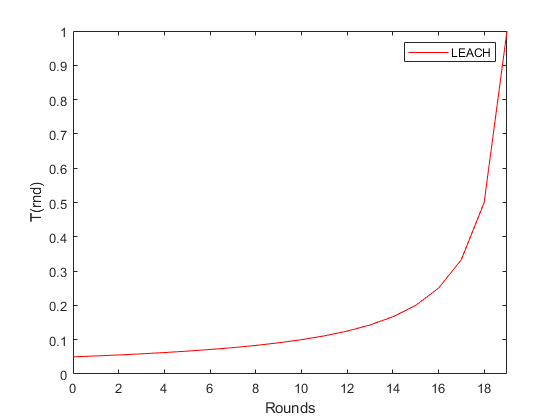
\includegraphics[scale=0.9]{Images/LEACHplot.png}
    \caption{Value of T(n) over one cycle with $P=0.05$}
    \label{fig:LEACHplot}
\end{figure}

\noindent After cluster heads have been chosen for a round it works like a regular LEACH protocol. All other nodes simply connect to whichever cluster head is closest, which is the cluster head that provides the strongest signal. This can be done with a CSMA MAC protocol that works by letting all nodes listen if there is some signal already broadcasting. If there is, the node waits a randomly generated amount of time until listening and trying again; if there is no signal, then it broadcasts and tries to connect to the nearest cluster head. The cluster head then assigns a TDMA schedule to each of it sub-nodes so that each node knows exactly which time window it is supposed to broadcast on.
Finally, as soon as clusters have been formed the cluster heads starts relaying data from it's connected nodes to the sink. When all the data has been received by the cluster head, it performs signal processing functions to compress the data into a single signal. For example, if the data are audio or seismic signals, the cluster-head node can beamform the individual signals to generate a composite signal \cite{heinzelman2000energy}.

\subsection{Sink Movement and Data Flow}
\label{subsec:sinkDataFlow}
% MAKE SURE THE MIXED INTEGER THINGY IS EXPLAINED IN MODEL DESCR
The equations governing the energy and data aggregation dynamics of each node in the system are derived from \cite{heinzelman2000energy} and are expressed as
\begin{flalign}
    E_{Tx}(b_{tx},d) &= E_{elec}b_{tx}+ E_{amp}b_{tx}d^{2} \\
    E_{Rx}(b_{rx}) &= i(E_{elec}+E_{DA})b_{rx} \\
    \Psi &= E_{Tx} + E_{Rx} - E_{gen}
\end{flalign}
where $b$ is amount of bits either transmitted ($tx$) or received ($rx$), $d$ is the distance between transmitter and receiver and $i$ is the number of nodes connected. $E_{Tz}$ and $E_{Rz}$ represent energy consumed for transmission and receiving respectively, $E_{gen}$ represent energy generated, and $\Psi$ represents the sum of these. $E_{elec}$, $E_{amp}$ and $E_{DA}$ are constants related to power circuit consumption.
Here, a CH performs both transmission and reception while non CHs only do transmitting. Each node is also able to stochastically generate a relatively small amount of energy during each time step. \newline

\section{Control Strategies}
\label{sec:ctrlstrategies}
\noindent In order to achieve a model based controller for a multi-variable system with two contradicting economic goals, multiple optimal control methods were considered. To determine the feasibility of the methods, a study of their respective advantages and limitations was conducted.\newline

\noindent Three popular model based optimal control methods were considered. These were MPC, dynamic programming (DP) and linear quadratic regulation (LQR). All these methods work by calculating an optimal sequence of control steps into the future, where the optimal sequence is defined by an objective function. \cite{grune2019dynamic}.\newline

\noindent DP calculates a global optimum via backward calculation. This means that each optimization problem starting from the horizon requires the prior optimization problems leading up to it to be defined \cite{grune2019dynamic}. Due to the stochastic dynamics and nonlinearities of the system, this would not be computationally feasible for controlling the entire system in practice. \newline

\noindent On the other hand, an online optimization method such as MPC or receding horizon LQR need only to act upon an approximation of the future states, consequently generating a sub-optimal but feasible solution. However, the receding horizon LQR is meant to be applied on linearly constrained models where the cost function is quadratic.\newline

\noindent Since the system at hand is nonlinear and subject to hard constraints such that
\begin{itemize}
    \item each node can only be controlled if it has attained CH role
    \item there is a limit to the amount of packets a node can send during a round
    \item there is a limit to the step length of the sink
\end{itemize}
the receding horizon LQR is not feasible. In contrast to this, constrained and nonlinear optimal control is what MPC famously excels at \cite{MPCbook}.\newline

\noindent A counterpart to model based control is the data driven approaches, such as simulated annealing, artificial neural networks (ANN) and RL. The simulated annealing method finds a global optimum after iterating over a period of time for a system that does not change. Since it is a possibility that the proposed control problem runs for an indefinite amount of time and has an ever changing optimum it is not feasible to use the simulated annealing algorithm. In this case, the use of an ANN is not feasible due to the reason that the desired movement of the sink is unknown. It is therefore not possible to calculate the error between the reference value and output value which is needed to update the weights of the ANN. \newline

\noindent An RL algorithm such as Q-learning and SARSA are model free, i.e. the model of the system is not needed for controlling the system. Instead, the system chooses actions and receives a user defined reward which is based on the chosen action. Since high PR and low EC is desired, there is an easy method to reflect the desired behaviour onto the reward given to the system. Thereby, the most feasible data driven controller to employ on the proposed system is RL. 

\section{MPC}
\label{nonlinMPC}
The nonlinear MPC (NMPC) control algorithm calculates its optimal control input sequence through numerically optimizing for a minimum or maximum value of an objective function $J^{*}=min/max\:C(x,u)$ \cite{MPCdimitry}. This is done in a receding horizon fashion, meaning that it only implements the first control action and then repeats the planning at every new sampling instant \cite{MPCbook}. By defining $J^{*}$ as a function dependent on an accurate model of the dynamics of the system as well as desired constraints on the solution, the system can be controlled towards a desired state with an optimal trajectory. In this case, optimality could be defined with regards to costs such as time or energy consumption. Another benefit of MPC is its capacity of handling multi-input multi-output systems that may have interactions between their inputs and outputs \cite{MatlabMPC}. However, one ought to take into consideration that with multiple variables comes an ever increasing computational load on the controller as the time complexity of the algorithm is $\mathcal{O}((nN)^{3})$ with $n$ and $N_c$ denoting the number of controlled inputs and the control horizon, respectively \cite{li2011application}.\newline

\noindent For a mathematical formulation of the NMPC problem, the stabilization problem for a systems described by a nonlinear set of
equations can be considered as
\begin{equation}
\label{ss-dynamic}
    x(k+1) = f(k, x(k), u(k), d(k)),\; x(0) = x_{0}
\end{equation}
Subject to state and input constraints
\begin{align}
     u(k) \in \mathcal{U}, \forall k\geq0 \; x(k) \in \mathcal{X}, \forall x \geq 0
\end{align}
Where the set of feasible input values is denoted by $\mathcal{U}$ and the set of feasible states is denoted by $\mathcal{X}$. For solving the optimization problem, it is assumed that $\mathcal{X}$ and $\mathcal{U}$ satisfy the following assumptions \cite{findeisen2002introduction}:
\begin{itemize}
    \item $\mathcal{U}$ is compact, $\mathcal{X}$ is connected and $(0,0)\in\mathcal{X}\times \mathcal{U}$
    \item The vector field $f$ is continuous and satisfies $f(0,0) = 0$
    \item The system \ref{ss-dynamic} has an unique continuous solution for any initial condition in the region of interest and any piecewise continuous and right continuous input function
\end{itemize}

\noindent For $J$, the standard quadratic form is the simplest and most often used one and can be described as follows
\begin{equation}
    Minimize\:J(x(k),u(k)),\: J=\sum_{k=0}^{K-1} x^{T}Qx + u^{T}Ru
\end{equation}
where Q and R denote positive definite, symmetric weighting matrices, $K$ is the control horizon length in discrete time steps, $x(k)$ is the system state vector at discrete time step $k$, $u(k)$ is the control input vector at discrete time step $k$.\newline

\noindent $J$ would also be subject to constraints for $k\in[0,\hdots,T-1]$ with the following forms
\begin{align}
    \mathcal{A}x(k) &+\mathcal{B}u(k)\leq \phi, \phi(k)  \label{leqeq}\\
    \mathcal{A}_{eq}x(k) &+\mathcal{B}_{eq}u(k) = \phi_{eq}, \phi_{eq}(k) \label{eqeq}
\end{align}
\noindent Here, $\phi$ and $\phi_{eq}$ are stated as either constants or dynamic vectors.

\subsection{Mixed-Integer Nonlinear Programming}
Mixed-Integer Nonlinear Programming (MINLP) problems are defined as those where some or all of the decision variables are only allowed to be integers. This is typically required in a range of real world applications in allocation and planning problems where the discrete variables represent quantities and require integer values for the solution. \newline

\noindent A common method of solving for integer representations of the decision variables is by using the "Branch and Bound" method. It works by initially finding the optimal solution to a relaxation of the problem without the integer constraints, via standard linear or nonlinear optimization methods. Thus, it results in a greater chance that the problem satisfies the previously stated assumptions. The method then branches out from the non-integer solution by creating several more tightly constrained sub-problems around the optimal point to find a solution that satisfies all the integer constraints \cite{frontlineSolversMIP}.\newline





\section{RL Theory}
 In a RL algorithm, e.g. Q-learning and SARSA, the so called agent learns without labeled data by executing actions $a$ from a pre-detemined action set $\mathcal{A}$ such that $a \: \in \: \mathcal{A}$. After performing the action, the agent evaluates the outcome of the action based on rewards, $R_t \: \in \: \mathcal{R} \: \subset \mathbb{R}$, from the environment where $\mathcal{R}$ is the set of rewards. The objective is to maximize the reward that the agent gains after each episode, i.e. after every iteration of the entire algorithm. The agent starts from an arbitrary initial state and receives a new state from the environment after performing an action. If the action is desired the agent will also receive a positive reward and vice versa, see Figure~\ref{fig:RLoverview}. The maximum reward that the agent can receive is determined by solving the Bellman equation which is the sum of the reward that the system obtains immediately by taking the action and the amount of future rewards that the agent can receive at the new state \cite{sutton2018reinforcement}. Further, in order to enable a trade off between exploitation of maximizing reward and exploration of the environment for the agent, a probability of $\epsilon$ is introduced for taking a random action. $\epsilon$ is the exploration rate and the agent will take a random action with a probability of $\epsilon$ \& will take the action that yields the highest reward with a probability of $1-\epsilon$. This method to explore the environment is needed due to that there could be sub-optimal states and is called $\epsilon$-greedy exploration. 

\begin{figure}[H]
  \centering
  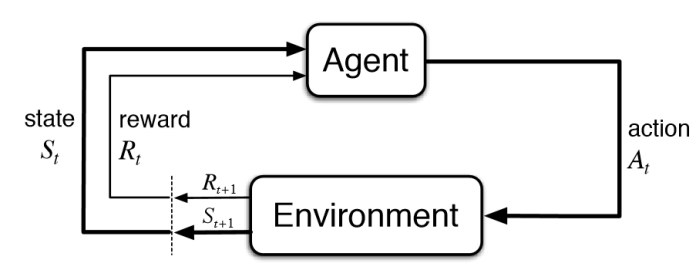
\includegraphics[width=0.9\textwidth]{Images/RLoverview.jpg}
  \caption{Overview of reinforcement learning algorithm \cite{sutton2018reinforcement} } 
  \label{fig:RLoverview} 
\end{figure}

\subsection{Q-learning}
\noindent  Q-learning is an RL algorithm that is model free. The algorithm finds the best action for a state by solving the Bellman equation stated in Equation \ref{eq:bellman}.

\begin{equation}
\label{eq:bellman}
    Q(s,a) = r + \gamma \max_{a'} Q(s',a')
\end{equation}

\noindent Here $Q(s,a)$ is called the quality-value (Q-value) and is the action-state value for a given state and action, $r$ is the immediate reward of an action, $\gamma$ is the discount factor for future states and $\max_{a'} Q(s',a')$ is the maximum future Q-value that can be obtained with a new action $a'$ given a new state $s'$. Thereby, Equation \ref{eq:bellman} states the immediate reward of an action and the maximum reward that the agent can receive when the agent has entered a specific state. The idea behind Q-learning is to iteratively update the Q-values, i.e. $Q(s,a)$, for every state-action pair such that it converges towards the optimal Q-value, $Q^*(s,a)$. At each iteration step, the Q-value is updated as in Equation \ref{eq:QValueIter} \cite{sutton2018reinforcement}.

\begin{equation}
\label{eq:QValueIter}
    Q_{t+1}(s_t,a_t)=Q_{t}(s_t,a_t)+\alpha(r_{t+1} + \gamma \max_{a} Q_t(s_{t+1},a)-Q_{t}(s_t,a_t))
\end{equation}

\noindent In this case $Q_{t+1}(s_t,a_t)$ is the updated Q-value from the previous Q-value $Q_{t}(s_t,a_t)$ and $\alpha$ is the learning rate which determines how much the difference between the new Q-value and the old Q-value affects each iteration step. The agent updates the Q-value with Equation \ref{eq:QValueIter} by randomly choosing actions from the action set with an $\epsilon$ probability and by choosing the action that the agent predicts would yield the most reward with a probability of $1-\epsilon$.

\subsection{Deep Q-Network}

The main disadvantage with the Q-learning algorithm is that the agent needs to step through every state-action pair multiple times to get a reasonable Q-value for all state-action pairs. Therefore, it becomes rapidly infeasible to solve the problem in a timely manner when the amount of states and actions are increased due to the curse of dimensionality. A RL algorithm that is more suitable for a large number of states and actions is deep Q-networks (DQN) which is an extension of the Q-learning algorithm.\newline

\noindent Instead of naively updating the Q-value when the agent reaches a state-action pair, the DQN algorithm approximates the Q-value of the state-action pair with a neural network (NN). The role of the NN is to map the states of the environment with the action that is optimal for the agent to take. In other words the NN determines which action is the most optimum, i.e. has the highest Q-value, for a specific state \cite{silver2013DQN}. \newline 
\newline
\noindent To train the agent, there is a need for expressing the difference between the prediction of the NN and the actual target value mathematically. The agent's loss is a value that is a quantitative measure of how good a prediction is. By using an optimizer the loss as a mean absolute error (MAE), and thereby also the NN's prediction error, is minimized. Equation \ref{eq:mse} depicts the MAE where $n$ is the amount of data points to be optimized for.   

\begin{equation}
    \label{eq:mse}
    MAE = \frac{1}{n}\sum^{n}_{t=1}(loss) 
\end{equation}

\begin{equation*}
         where \hspace{0.25cm} loss =  |\underbrace{r + \gamma \max_{a_{t+1}} Q_t(s, a_{t+1})}_{Target} - \overbrace{Q_{t}(s_t,a_t)}^{Prediction}|
\end{equation*}

\noindent The optimizer does all of the work of minimizing the loss by tuning the weights of the NN based on the absolute error between the target and the NN output. This leads to a converging Q-value and a decreasing loss. After the best action was performed and the weights of the NN are updated the DQN algorithm follows the Q-learning algorithm until the next occasion an action is to be selected. 

\subsection{Neural Network}

A neural network is a field within machine learning. The main usage of a NN is to find a pattern between a given input and an output by mimicking the biological structure of a brain with its dendrites and synapses \cite{SiddiqueNH2013Ciso}. In a NN the basic building block is called a neuron and by connecting a number of neurons a NN is formed. As seen in Figure \ref{fig:NNoverview} the neurons are ordered in layers in which the first layer is the input layer and the last layer is the output layer. Each neuron in the input layer corresponds to one variable, i.e. one input, and between the input layer \& the output layer there are an arbitrary amount of hidden layers. Additionally every edge, i.e. every connection between two neurons, has a weight associated with it. It is these weights that determine the output of a neuron based on a given input. \newline       

\begin{figure}[h]
    \centering
    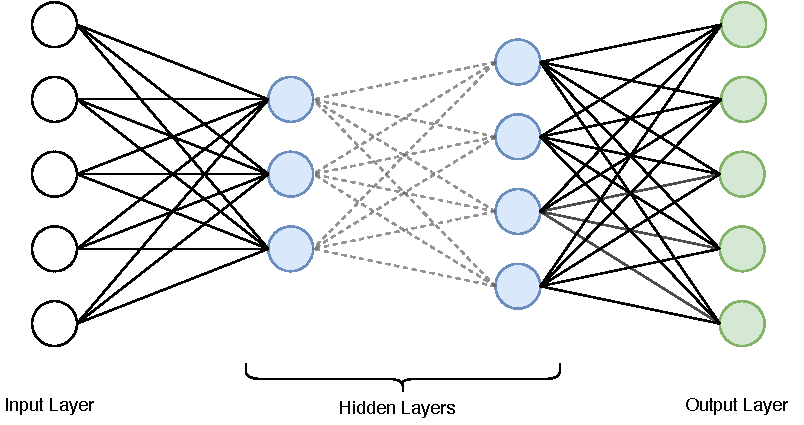
\includegraphics[scale=1]{Images/NNoverview.pdf}
    \caption{Overview sketch of a NN}
    \label{fig:NNoverview}
\end{figure}

%\vfill \break
\noindent The learning process starts when data is provided to the input layer. By using the edge's weights the NN calculates the output value of all the neurons in the output layer. The NN then uses the difference between the calculated output \& the expected output to update the weights via an optimization algorithm in order to make better predictions in the future. This process of improving the weights is called error backpropagation. The role of the optimization algorithm is to minimize the loss of the NNs predictions by updating the edge's weights based on gradient descent \cite{SiddiqueNH2013Ciso}.  

\subsubsection{Remember, Memory and Replay}
\noindent One major issue with the DQN algorithm is that the NN has a tendency of forgetting what was learned previously when it overwrites them with new experiences. Therefore, a remember function needs to be used to append the previous observations and experiences onto an array named memory. After every action, the agent replays a number of randomly chosen experiences from its memory and the weights of the NN are once again fitted based on these experiences \cite{lin1992self}. 


\section{Software Tools}
\label{sec:softwaretools}
Some parts required for the controllers' basic structure were already available through libraries. This section presents options considered for the tasks.


\subsection{Optimization Tool}
A couple of different libraries were considered for simplifying and streamlining the process of solving the optimization problems related to the optimal control approach. \newline
\newline
\noindent \textbf{CasADi} is an open-source tool for nonlinear optimization and algorithmic differentiation.
It facilitates rapid — yet efficient — implementation of different methods for numerical optimal control, both in an offline context and for nonlinear model predictive control (NMPC) \cite{Andersson2018}. The tool is compatible with both Matlab and Python.\newline

\noindent \textbf{GEKKO} is a Python package for machine learning and optimization of mixed-integer and differential algebraic equations. It is coupled with large-scale solvers for linear, quadratic, nonlinear, and mixed integer programming (LP, QP, NLP, MILP, MINLP). Modes of operation include parameter regression, data reconciliation, real-time optimization, dynamic simulation, and nonlinear predictive control \cite{beal2018gekko}.\newline

\noindent Both libraries offer sufficient means for continuously solving non-linear optimization problems. However, in the opinion of the authors at that moment, GEKKO offered far better support and guidance in the form of an active user forum and example material.

\subsection{Machine Learning Tool}
Two of the most established machine learning libraries that are compatible with Python are pyTorch and TensorFlow. Below follows a short description of both machine learning libraries. \newline
\newline
\noindent \textbf{PyTorch} is a deep learning framework that is based on Tourch \cite{paszke2017automatic}. It has a simple interface, is easily extendable and integrates into Python smoothly. The computational graph in pyTorch is updated dynamically which means that the graph is updated at runtime and hence it is easier to debug. \newline 
\newline
\noindent \textbf{TensorFlow} is an open-source library that can be used to build and train machine learning models \cite{tensorflow2015-whitepaper}. When using this library it is possible to add an abstraction level by building the model on an application programming interface (API) called Keras \cite{chollet2015keras}. Further, TensorFlow provides a vast range of material which aids the learning process.\newline   
\newline 
\noindent PyTorch and TensorFlow are both capable libraries and could solve the RL problem. Nevertheless, the Keras API which runs on top of TensorFlow had a larger community, better guidance and documentation. For setting up the WSN environment in a reinforcement learning context, the gym library from OpenAI provides a straightforward procedure to model the reward \cite{open160601540}.


%For controlling the mobile sink with RL, it was decided to run Keras on top of TensorFlow.

\chapter{Implementation}
\textit{In this chapter, detailed information of the design and implementation process of the WSN control system is provided based on what was recorded during the literature review. Furthermore, detailed theory of the two control strategies is discussed.}

\section{WSN Simulation Environment}
 In order to make unbiased comparisons between the two controllers' performances, all tests had to be executed in an identical simulation environment. Based on the grounds that the WSN simulation environment needed to mainly be energy-oriented to answer the research questions, there were not any ideal pre-built simulators. Instead it was decided to develop and build a WSN environment which focused on the energy consumption of the nodes in the WSN. The WSN environment was developed using the equations governing the energy \& data aggregation as stated in Subsection \ref{subsec:sinkDataFlow} and consisted of three classes together with a script for visualizing the environment. See Figure \ref{fig:WSNUML} for a UML representation of the WSN simulation environment. 

\begin{figure}
    \centering
    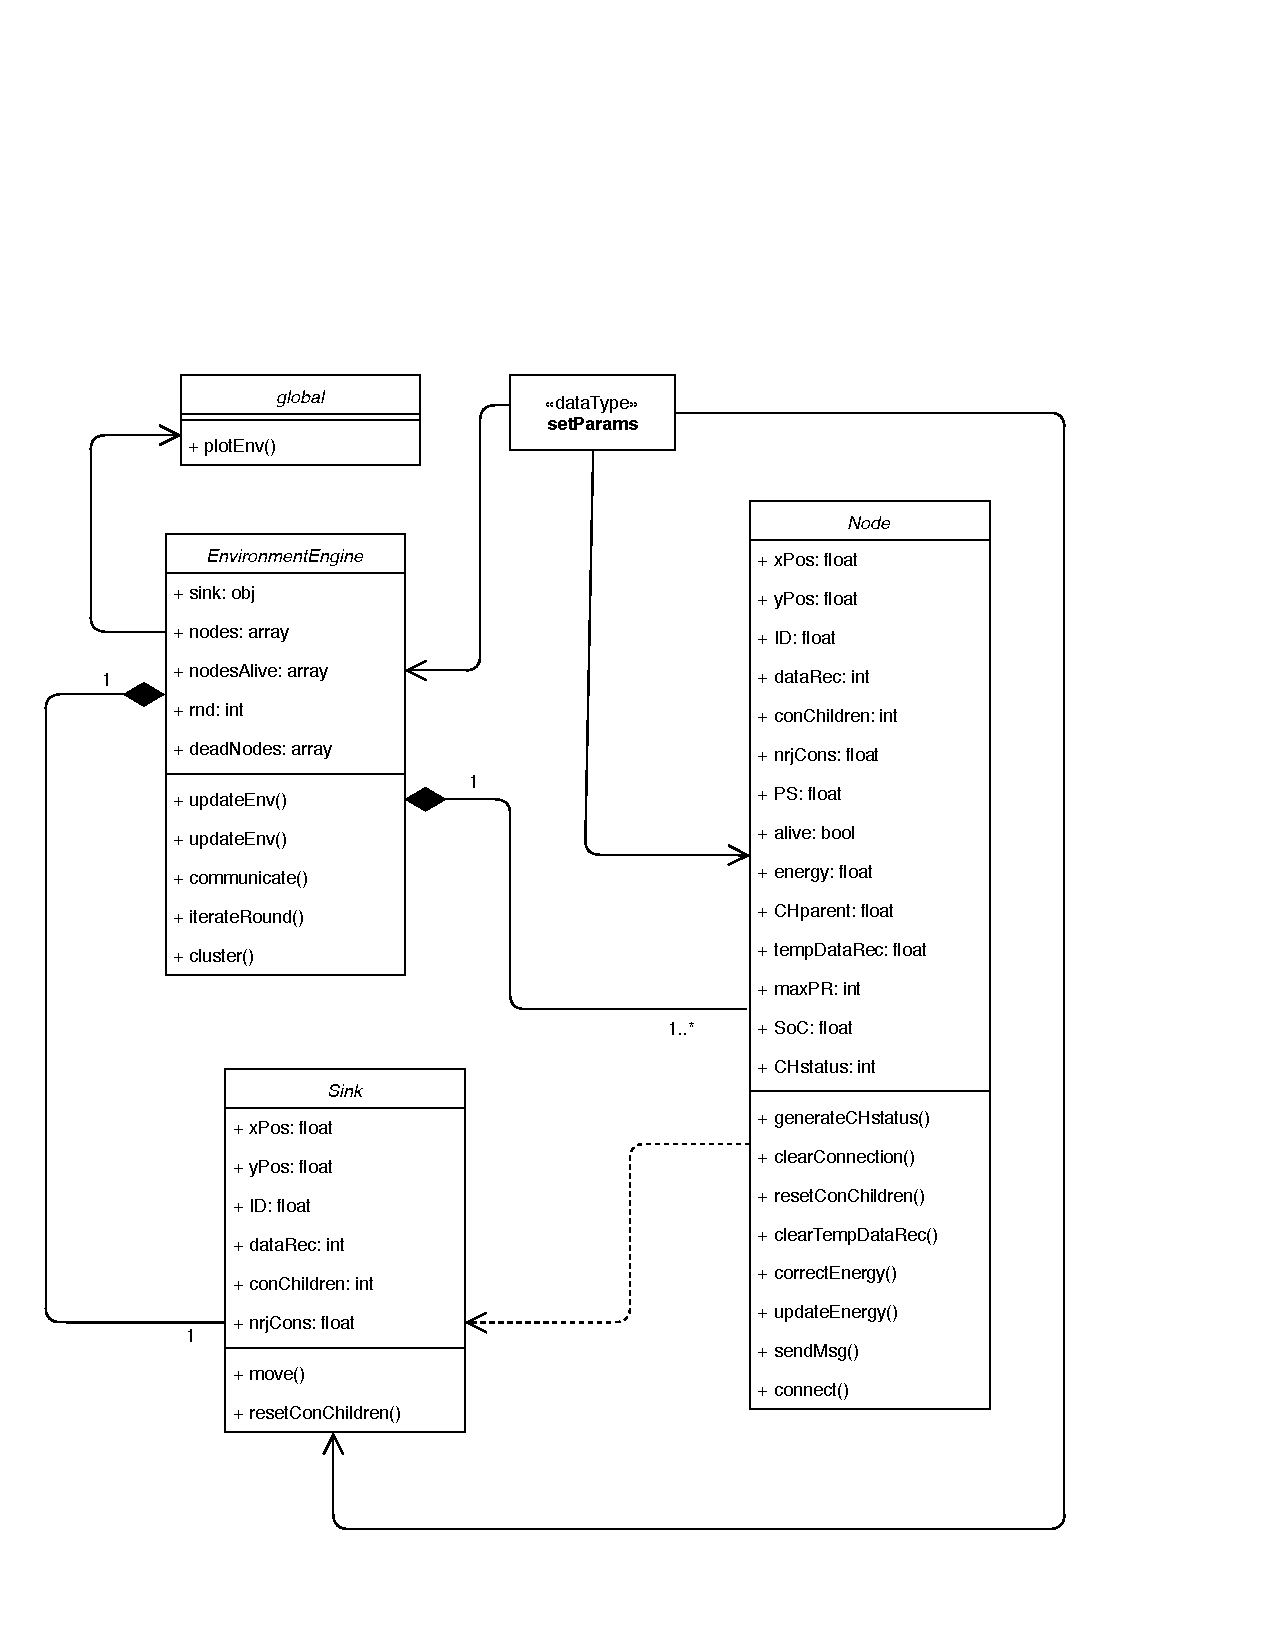
\includegraphics[scale=.7]{Images/WSNUML.pdf}
    \caption{UML of WSN simulation environment}
    \label{fig:WSNUML}
\end{figure}

 \subsection{Simulation Environment Architecture}
 \subsubsection{Sink}
 The mobile sink was represented as an object with the \verb!Sink! class. By using the size of the WSN environment the \verb!Sink! object was always placed in the middle when it was initiated. The most pivotal method of this class is named \verb!move()! which enabled movement of the sink in any direction.     

 \subsubsection{Node}
 The \verb!Node! class was used to represent one node in the simulation environment. When a node was created it required a node ID number, $x$- \& $y$-position and an initial energy level as input. After an instance of the node was created, methods such as \verb!generateCHstatus()!, \verb!connect()!, \verb!sendMsg()! and \verb!updateEnergy()! were utilized to decide whether the node's CH status, connect to the sink or another node, send data messages and update the node's energy after sending and/or receiving data respectively. 

 \subsubsection{EnvironmentEngine}
 \noindent The \verb!EnvironmentEngine! class had the responsibility of interlinking the different modules of the WSN environment. By holding onto one \verb!Sink! object and numerous \verb!Node! objects the \verb!EnvironmentEngine! class linked together the modules with its methods. The \verb!cluster()! method elected CHs, \verb!updateEnv()! method moved the sink \& changed the PR of the nodes, \verb!communicate()! method sent the messages between nodes \& nodes/sink and the \verb!iterateRound()! method was used to reset some attributes before the start of a new round.

\subsubsection{Main script}
To visualize the WSN and its performance, a function based on the \verb!Matplotlib! library was implemented. This function plotted the sink and the nodes in a 2D grid as well as which of the nodes were CHs. The performance of the controllers were depicted in real time as plots of energy consumed, amount of dead nodes and amount of data packets sent as a function of the current round. \newline

\noindent To simulate the behaviour of the system, the interaction of the classes were put in a loop designed to break if the environment engine detected 0 alive nodes. During each loop, three actions were repeated until network failure, see Figure \ref{fig:mainscriptflowchart}.
\begin{figure}
    \centering
    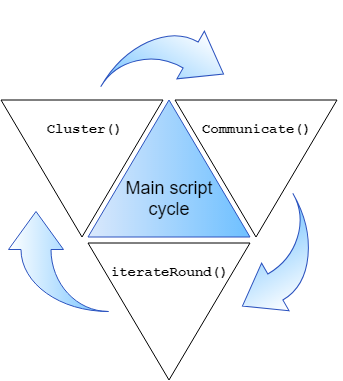
\includegraphics[scale = 0.45]{Images/mainscriptflowchart.png}
    \caption{Main script action sequence for each loop until network failure.}
    \label{fig:mainscriptflowchart}
\end{figure}
In order to control the network, each transmission round was split into a minor loop of a set number of time segments. During each time segment, each CH was allowed to execute \verb!sendMsg()! with a regulated amount of packages. \newline


\subsubsection{Distributed- Versus Random-Mode}
Two different settings were implemented in order to be able to choose whether the nodes should all begin with the same amount of energy or if they should begin with a randomized amount of energy. \verb!distr! signaled that each node would start with the same energy, while \verb!rand! meant that each node would start with $E=rand(1)\cdot Max\:energy$. The purpose of the random mode was to simulate a real world application where energy consumption, and generation, could be stochastic or favoured in certain areas.

\subsubsection{Environment Parameters}
\noindent Table \ref{tb:Envdesign} depicts the parameter values that were used during simulations.  

\begin{table}[h!]
    \centering
    \caption{Environment parameter choices}
    \label{tb:Envdesign}
    \begin{tabular}{ 
        l % left aligned column
        l % left aligned column
        *{3}{S[table-format=4.0]} % three columns with numeric data       
    }
        \toprule
        \textbf{Parameter} & \textbf{Value}  \\ 
        \midrule
        $x \: size$ & $100 \: m$ \\ \\[-1em]
        $y \: size$ & $100 \: m$ \\ \\[-1em]
        $Max \: energy$ & $0.05 \: J$ \\ \\[-1em]
        $E_{elec}$ & $ 50 \cdot 10^{-9} \: \frac{J}{bit}$ \\ \\[-1em]
        $E_{Tx}$ & $ 50 \cdot 10^{-9} \: \frac{J}{bit}$ \\ \\[-1em]
        $E_{Rx}$ & $ 50 \cdot 10^{-9} \: \frac{J}{bit}$ \\ \\[-1em]
        $E_{amp}$ & $ 10^{-10} \: \frac{J}{bit \cdot m^{2}}$ \\ \\ [-1em]
        $E_{DA}$ & $ 50 \cdot 10^{-9} \: \frac{J}{bit}$ \\ \\[-1em]
        $Time\:segments$ & $10$\\ \\[-1em]
        $Mode$ & $'distr'\: or \: 'rand'$\\ \\[-1em]
        \bottomrule
    \end{tabular}
\end{table}



\section{BLEACH}
The broadening of the LEACH protocol equation, now called BLEACH (Broadened LEACH), was to have the term $SoC$ included. Here, $SoC\in[0,1]$ was defined as the percentual amount of energy stored in the node.
\begin{equation}
    SoC = \frac{E_{current\:battery}}{E_{max\:battery}}
\end{equation}
Several requirements and soft goals were created for the BLEACH equation.
\begin{enumerate}
    \item The equation shall be able to produce CHs at any round as long as there are nodes are alive which have elected during the current episode
    \item The influence of the $SoC$- and round-dependency shall be dynamic and adjustable
    \item The equation shall only involve variables and parameters available to the individual node
    \item It would be beneficial if the amount of CHs relative to the total number of nodes is similar for each round
    \item It would be beneficial for the equation to function as regular LEACH when there is little to no difference in $SoC$
\end{enumerate}
\noindent If the established requirements for the expression was deemed as satisfied, the development process was to move on towards testing for analyzing of results, see Chapter \ref{ch:Methodology}.

\subsection{BLEACH Expression Design}
A direct coupling of the $SoC$ to the LEACH expression $T_{LEACH}$, see Equation \ref{leacheq}, would result in lowering the overall $T$-value among the nodes; as soon as energy runs low in the network, little to no CH roles would be produced. In response to this, the BLEACH expression was divided into two functions $S(n, SoC)$ and $R(n)$, see Equation \ref{SandR}. One term was to be dependant on the $SoC$, and the other only dependant on the current round. 
\begin{equation}
    \label{SandR}
    T_{BLEACH}(rnd, SoC) = (1-f)\cdot S + f\cdot R
\end{equation}
The weight factor $f$ was introduced in order to regulate the total value of $T_{BLEACH}$. To retain the behaviour of the former equation, both
$S$ and $R$ were based on the original expression. \newline
The following definitions were formed
\begin{align}
    \label{SandRexpanded}
    S &= h_s\frac{P}{1-P(rnd\,mod\frac{1}{P})}SoC = h_s\cdot T_{LEACH} \cdot Soc\\
    R &= h_r\cdot C \cdot \frac{P}{1-P(r\,mod\frac{1}{P})} = h_r \cdot C \cdot T_{LEACH}\\
    C &= \frac{1}{1-(1-f)\big(\frac{P}{1-P(r\,mod\frac{1}{P})}\big)} = \frac{1}{1-(1-f)T_{LEACH}}
\end{align}
\noindent A mechanism was required to ensure that CHs were chosen with a similar distribution despite energy being low on all nodes. This was the purpose of the additional parameter $h_s$ in $S$ and the additional factor $C$ in $R$. 
$C$ works by gradually nullifying $f$ towards the end of the cycle. For example, if $h_r = 1$ and $r = \frac{1}{P}-1$ (the last round index of the cycle), we have that
\begin{align}
    C = \frac{1}{f} \\
    f\cdot R = f\cdot C \cdot \frac{P}{1-P(r\,mod\frac{1}{P})} = T_{LEACH}\\
\end{align}

thus making sure that $T\geq1$ is guaranteed for the remaining nodes at the last round. However, a value of $R\geq1$ is not desired for all nodes at the final round; if each node was guaranteed to become a CH during each cycle, the $SoC$-prioritization would serve no purpose. Therefore, the factor $h_r$ was introduced to control the impact of $R$ so as to keep $T_{BLEACH}(\frac{1}{P})$ below 1 for nodes with $SoC$ below a certain value.\newline

\noindent The parameter $h_s$ decides in which range $S$ can vary. If $h_s\not> 1$, then $T_{BLEACH}$ would assume lesser values than $T_{LEACH}$ at each round where $f\cdot C \leq f$ regardless of $SoC$, as seen in Equation \ref{h_sproof}.\newline
For $h_s,h_r = 1$
\begin{align}
    \label{h_sproof}
    T_{BLEACH} = f\cdot S + (1-f)\cdot R = &f\cdot T_{LEACH}\cdot SoC + (1-f)\cdot C \cdot T_{LEACH} \\
    for\;&SoC\in[0,1], \nonumber \\
    &\Downarrow \nonumber \\
    T_{BLEACH} = T_{LEACH}(1&+f(SoC-1))\leq T_{LEACH} \nonumber
\end{align}

\noindent The expression modifications were continuously observed in MATLAB to evaluate their behaviour with respect to the previously mentioned requirements. The observations where made at different stages of a cycle at different levels of $SoC$, see Figure \ref{fig:B_LEACHplots}. 


\begin{figure}
    \centering
    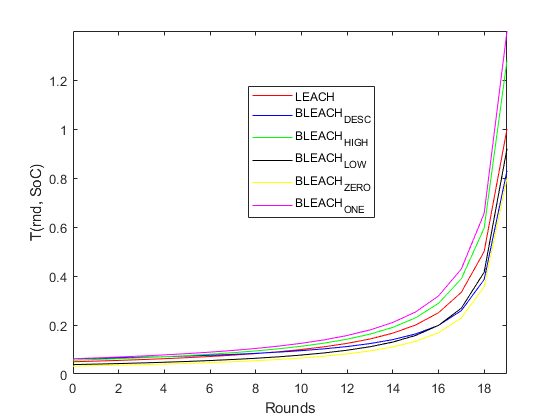
\includegraphics[scale=0.9]{Images/B_LEACHallPlots.png}
    \caption{Value of $T$ over one cycle for $P=0.05$, $f=0.8$, $h_s=3$ and $h_r = 0.8$ for LEACH and BLEACH with varying $SoC$. $BLEACH_{HIGH}$ represents a constantly high value of $SoC = 0.8$, $BLEACH_{LOW} \Rightarrow SoC = 0.2$, $BLEACH_{ONE} \Rightarrow SoC=1$, $BLEACH_{ZERO} \Rightarrow SoC=0$, and $BLEACH_{DESC}$ plots a decreasing value of $SoC \in [1 0]$. $T_{BLEACH}$ exhibits a behaviour similar to $T_{LEACH}$. However, the values are distributed on both sides of the original depending on the node's $SoC$.}
    \label{fig:B_LEACHplots}
\end{figure}

\subsubsection{Simplified BLEACH}
As an alternative to the more complex former expression, an additional approach was offered.
As previously discussed, there was reason to believe that a $T$-value varying between values close to $T_{LEACH}$ depending on $SoC$ was to be beneficial. This solution works by implementing a look-up table of size $100\times L_{cycle}$, where $L_{cycle}$ is the amount of rounds in a cycle. The table is filled with scaled versions of $T_{LEACH}$ such that

\begin{align}
\hspace{-1.25cm}
\tiny
    \begin{bmatrix}
        (1-spread)\cdot T_{LEACH, n=1} & (1-spread)\cdot T_{LEACH, n=2} &\hdots& (1-spread)\cdot T_{LEACH, n=L_{cycle}} \\
        (1-spread+step)\cdot T_{LEACH, n=1} & (1-spread+step)\cdot T_{LEACH, n=2} &\hdots& (1-spread+step)\cdot T_{LEACH, n=L_{cycle}}\\
        (1-spread+2\cdot step)\cdot T_{LEACH, n=1} & (1-spread + 2\cdot step)\cdot T_{LEACH, n=2} &\hdots& (1-spread +2\cdot step)\cdot T_{LEACH, n=L_{cycle}}\\
        \vdots & \vdots & \ddots & \vdots \\
        (1+spread)\cdot T_{LEACH, n=1} & (1+spread)\cdot T_{LEACH, n=2} &\hdots& (1+spread)\cdot T_{LEACH, n=L_{cycle}}
    \end{bmatrix} 
\end{align}
where $step = \: 2 \frac{spread}{100}$ and $spread$ is the range of which the $T$-value is able to stray from the standard value of $T_{LEACH}$. The interval $[spread, spread+step, \hdots, spread+99\cdot step]$ is divided into 100 elements where each element corresponds to a scaling of $T_{LEACH}$, which is seen as a row in the table. In turn, each row corresponds to a specific value of $SoC$. For example, $spread=0.3$ and $SoC = 0.80$ would correspond to row $\# \: 80$ in the table which results in $(1-0.3+79\cdot step)\cdot T_{LEACH} = 1.174\cdot T_{LEACH}$.
The resulting spectrum of possible $T$-values can be seen in Figure \ref{fig:oBLEACH}.
\begin{figure}
    \centering
    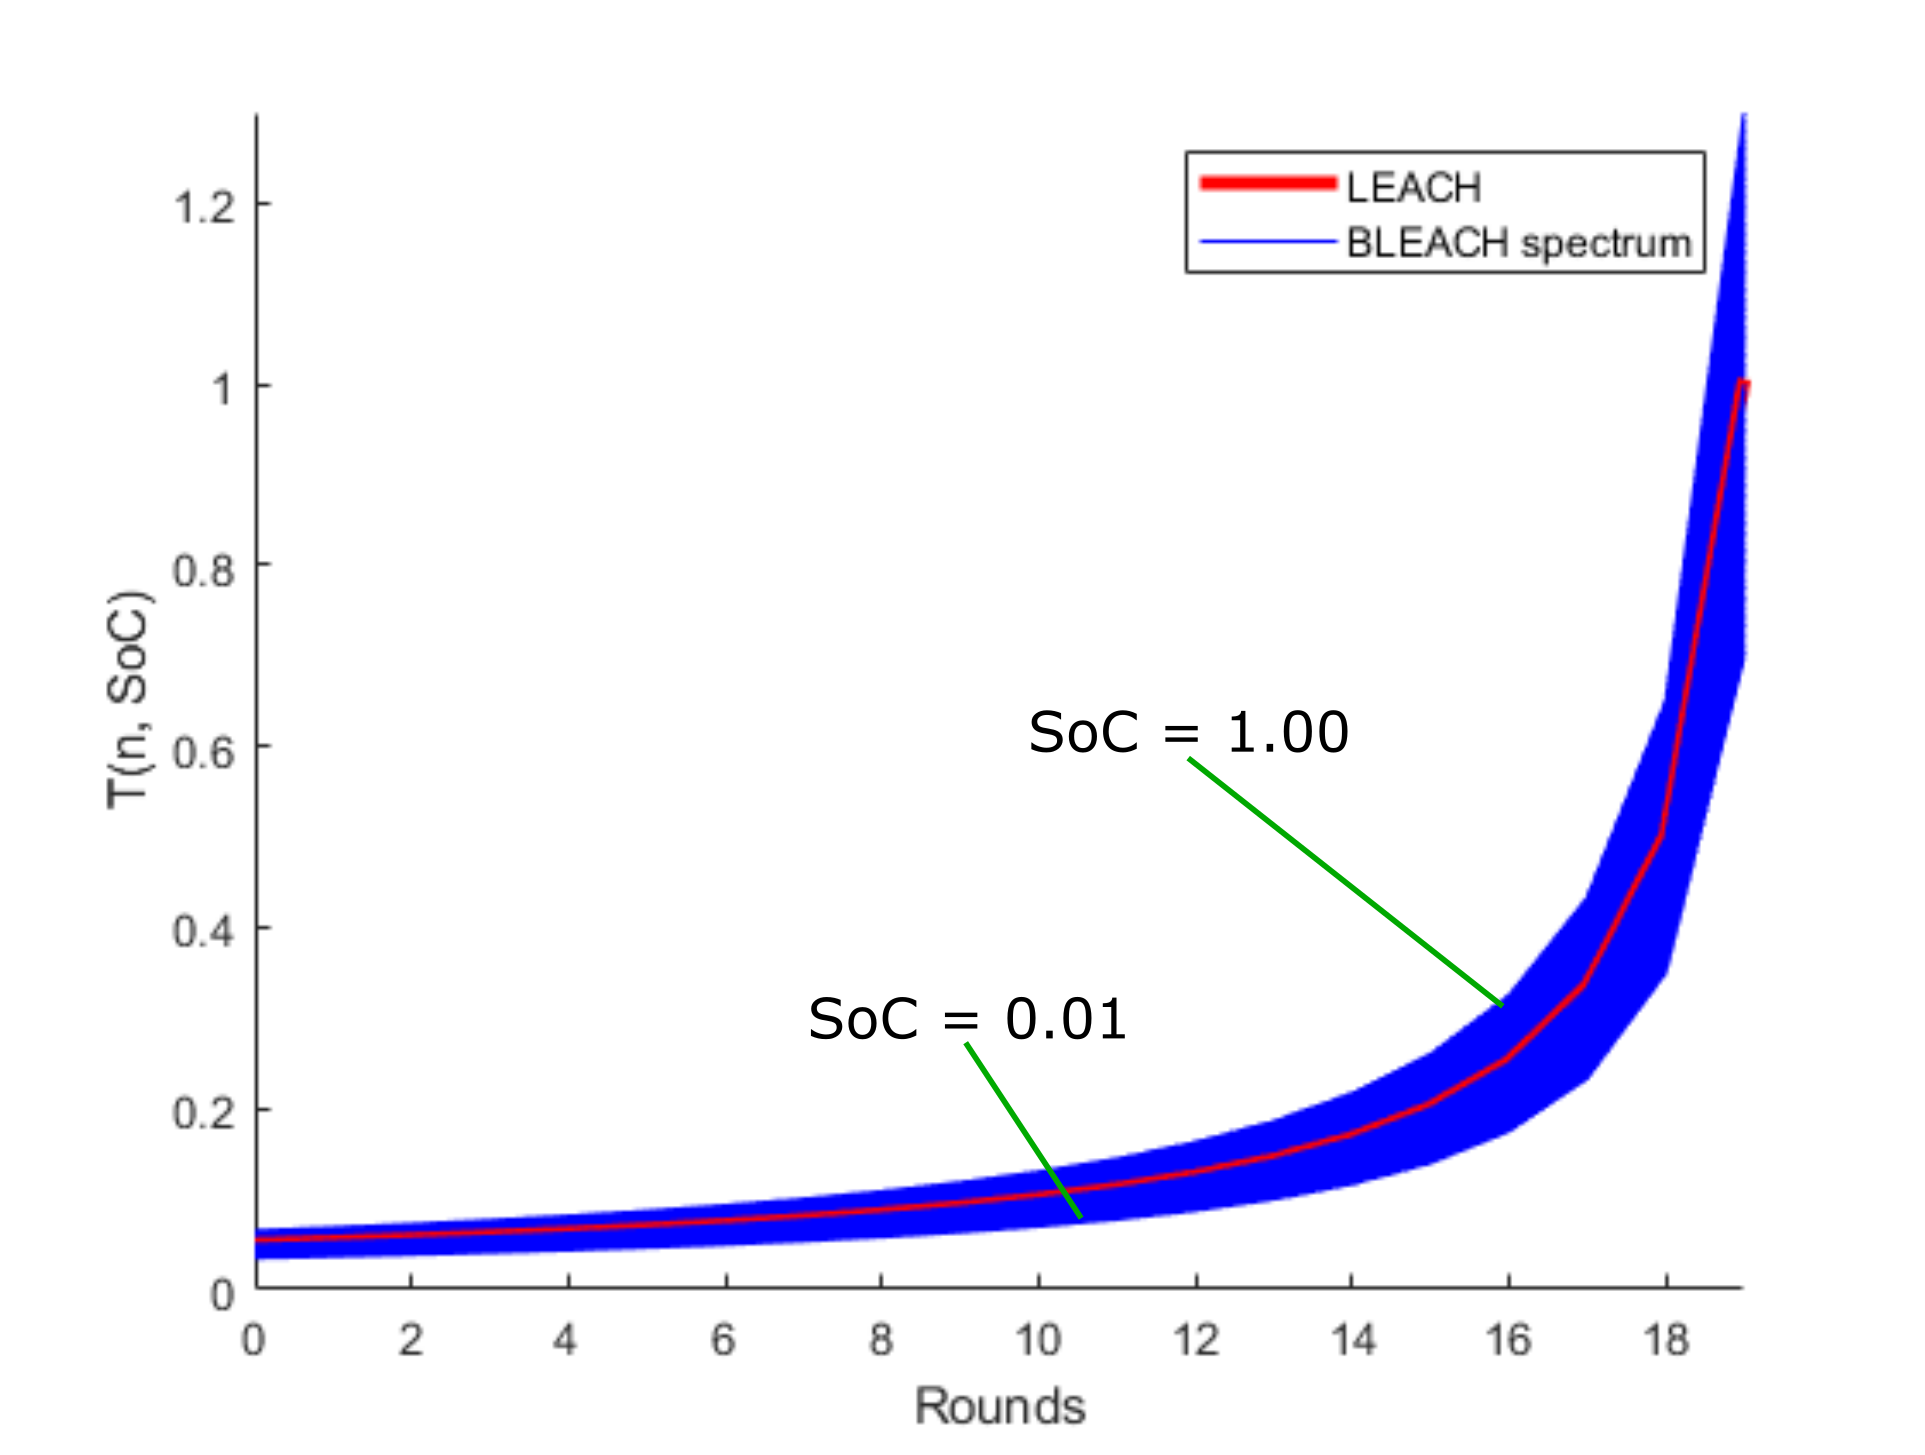
\includegraphics[scale=0.3]{Images/oBLEACH.png}
    \caption{Solution space for all possible $T$-values over a cycle for the simplified BLEACH-method. As demonstrated, $SoC\geq 0.5$ results in $T\geq T_{LEACH}$.}
    \label{fig:oBLEACH}
\end{figure}


\section{MPC Design}
Due to the advantages discussed in Chapter \ref{ch:LitReview}, NMPC was chosen as the model-based control strategy for the project. The proposed architecture of the controller-environment interaction can be seen in Figure \ref{fig:NMPCarchi}. Since the controller was to be implemented in a simulation environment devoid of any control disturbances or measurement noise, the state estimator part (as presented in \cite{findeisen2002introduction}) was not included.
\begin{figure}
    \centering
    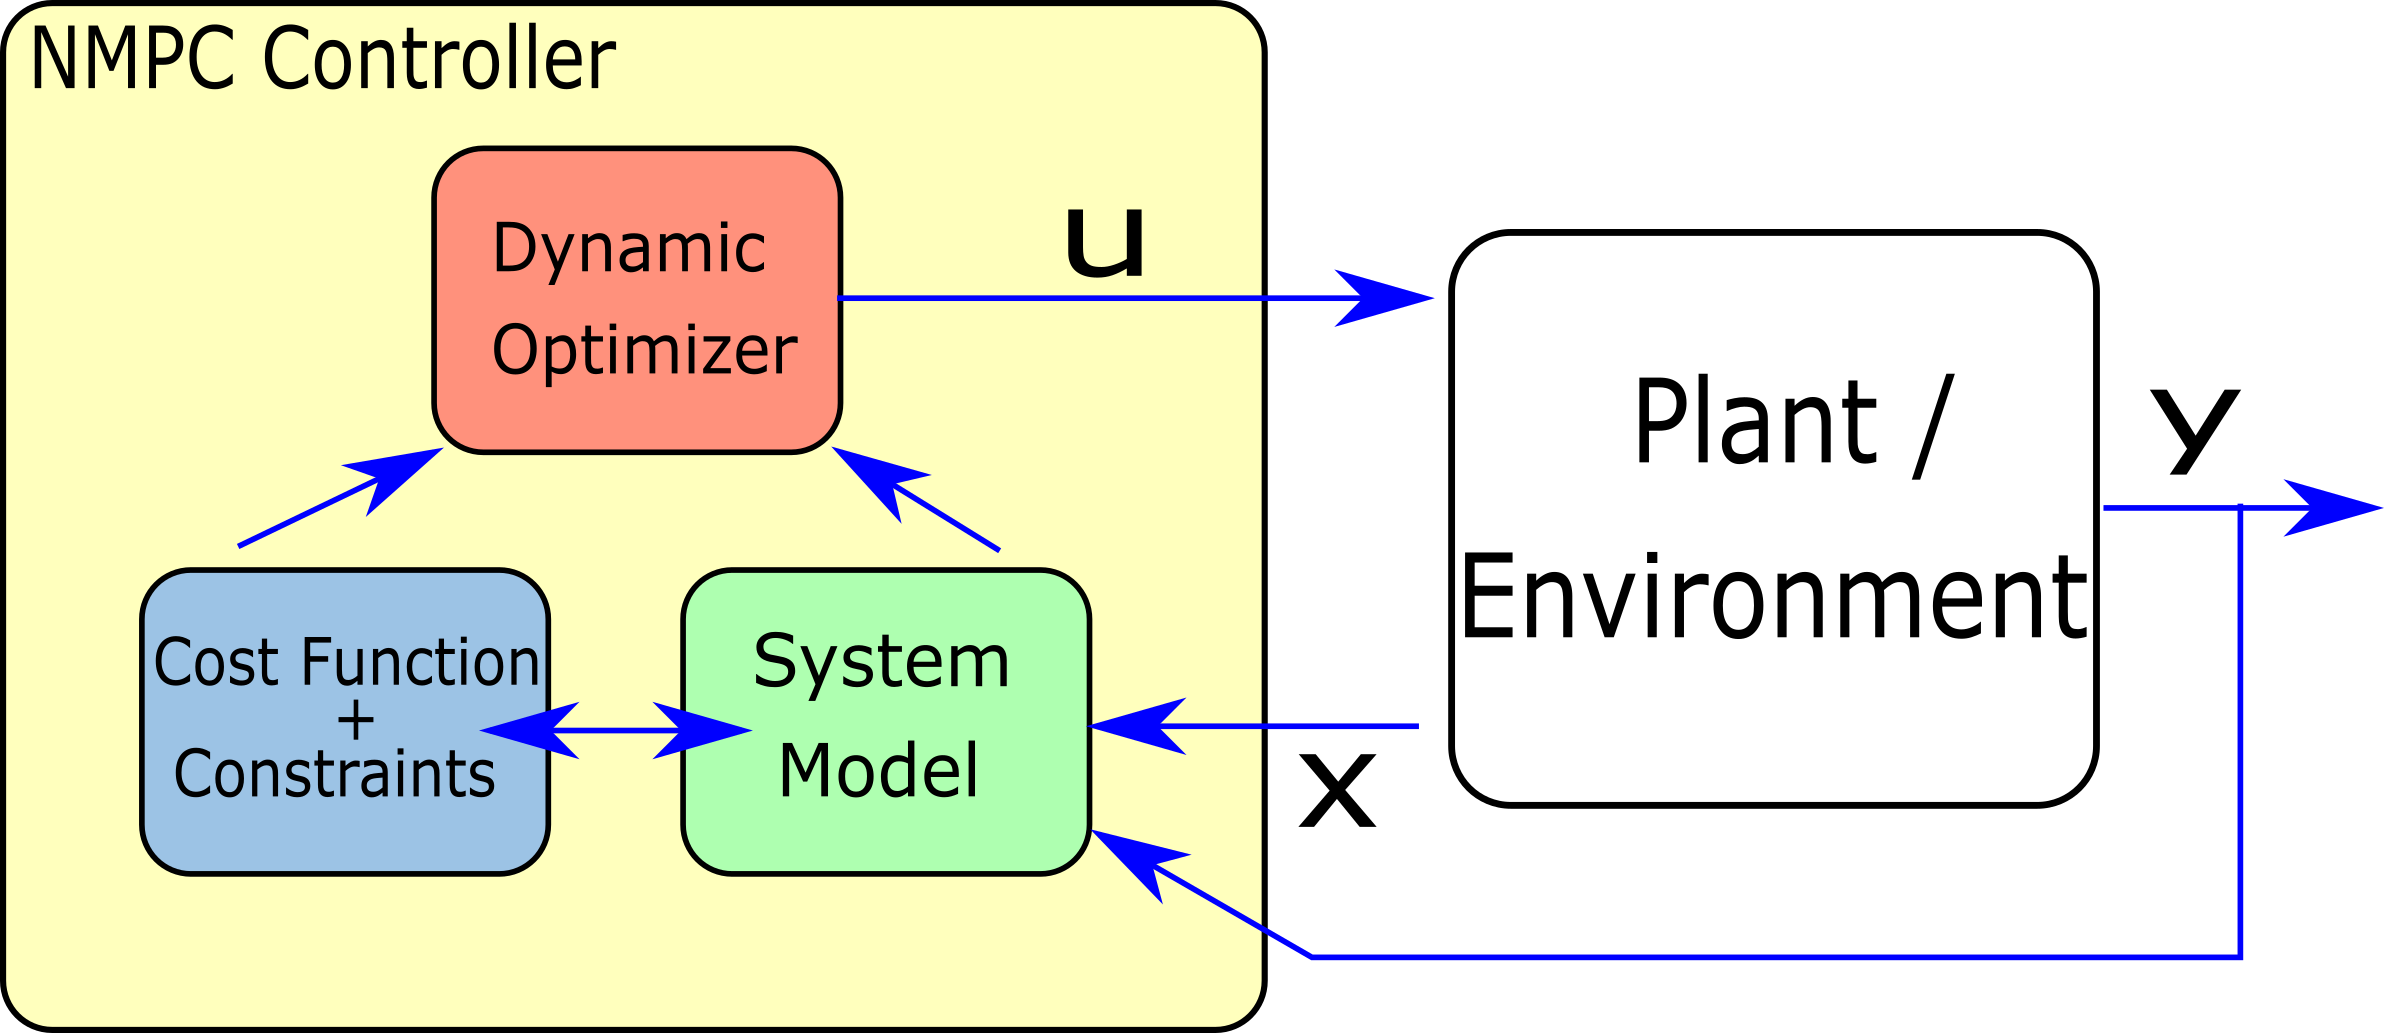
\includegraphics[scale=0.2]{Images/NMPCcontr.png}
    \caption{Basic NMPC control loop.}
    \label{fig:NMPCarchi}
\end{figure}

\noindent The complete optimal control problem was formulated with a mathematical model of the system. A corresponding MPC architecture with receding horizon was then designed and implemented with a chosen optimization tool. GEKKO was chosen over CasADi for this implementation due to its previously discussed benefits.\newline

\noindent The problem was to be solved by optimizing for a control sequence that minimizes a stated objective function $J$ depending on the two economic goals. Namely, the energy consumed and packets received by the sink. Energy consumed increases the cost while data received by the sink decreases it.
The state vectors \textbf{x}, \textbf{u} and \textbf{d}, representing states, control inputs, and disturbance, respectively are expressed in vector form as
\begin{align}
\label{x_k}
    \textbf{x} = [x_{sink}, y_{sink}, x_{1,\hdots,N}, y_{1,\hdots,N}, CHS_{1,\hdots,N}, PS_{1,\hdots,N}, EC_{1,\hdots,N}]^{T} \qquad x \in  \mathbb{R}^{5N+2}\\
    \textbf{u} = [\Delta x_{sink}, \Delta y_{sink}, PA_{1,\hdots,N}]^{T} \qquad u \in  \mathbb{R}^{N+2}\\
    \textbf{d} = [E_{gen,1\hdots,N}]^{T} \qquad d \in  \mathbb{R}^{N}
\end{align}

\noindent $N$ is the number of nodes and $(\Delta x_{sink}, \Delta y_{sink})$ is the change in position of the sink. The position of node $i,\:[1,...,N]$ nodes is assumed to be static. $PS_i$ is the amount of packets sent, $PA_i$ is a control input deciding how many packets to send each control step depending on the distance $d_i$ from each node $i$ to the sink, $EC_i$ is energy consumed, and $E_{gen}$ is a node's generated energy modeled as a disturbance. Cluster head status $CHS_i \in [0,1]$ is an indicator of whether the node has been chosen to be a cluster head or not which would decide if control is to be executed with regards to that node. \newline

\noindent As mentioned in Section \ref{nonlinMPC}, with an increasing number of nodes the dimension of the state space increases at a problematic rate. For example, 100 nodes with 5 controlled inputs, as well as a sink a sink with 2, over a horizon $K=10$ (the previously specified number of time segments per transmission round) would result in near $1.3\cdot10^{11}$ computations per control step.
To circumvent this, a strategy involving breaking down the optimization problem for the entire state space into minor optimization problems was deployed.\newline

\noindent As shown in Figure \ref{fig:splitctrl}, one lower layer optimization problem is stated for each node, with $x_{node},\:u_{node}$, as well as one upper layer for the sink with state vector, $x_{sink}, \: u_{sink}$. With this architecture, the $\mathcal{O}$-notation based on the previous example could be reduced to a worst case at approximately $100\cdot(5\cdot10)^{3}<1.3\cdot10^{7}$ computations per control step. 
\begin{figure}
    \centering
    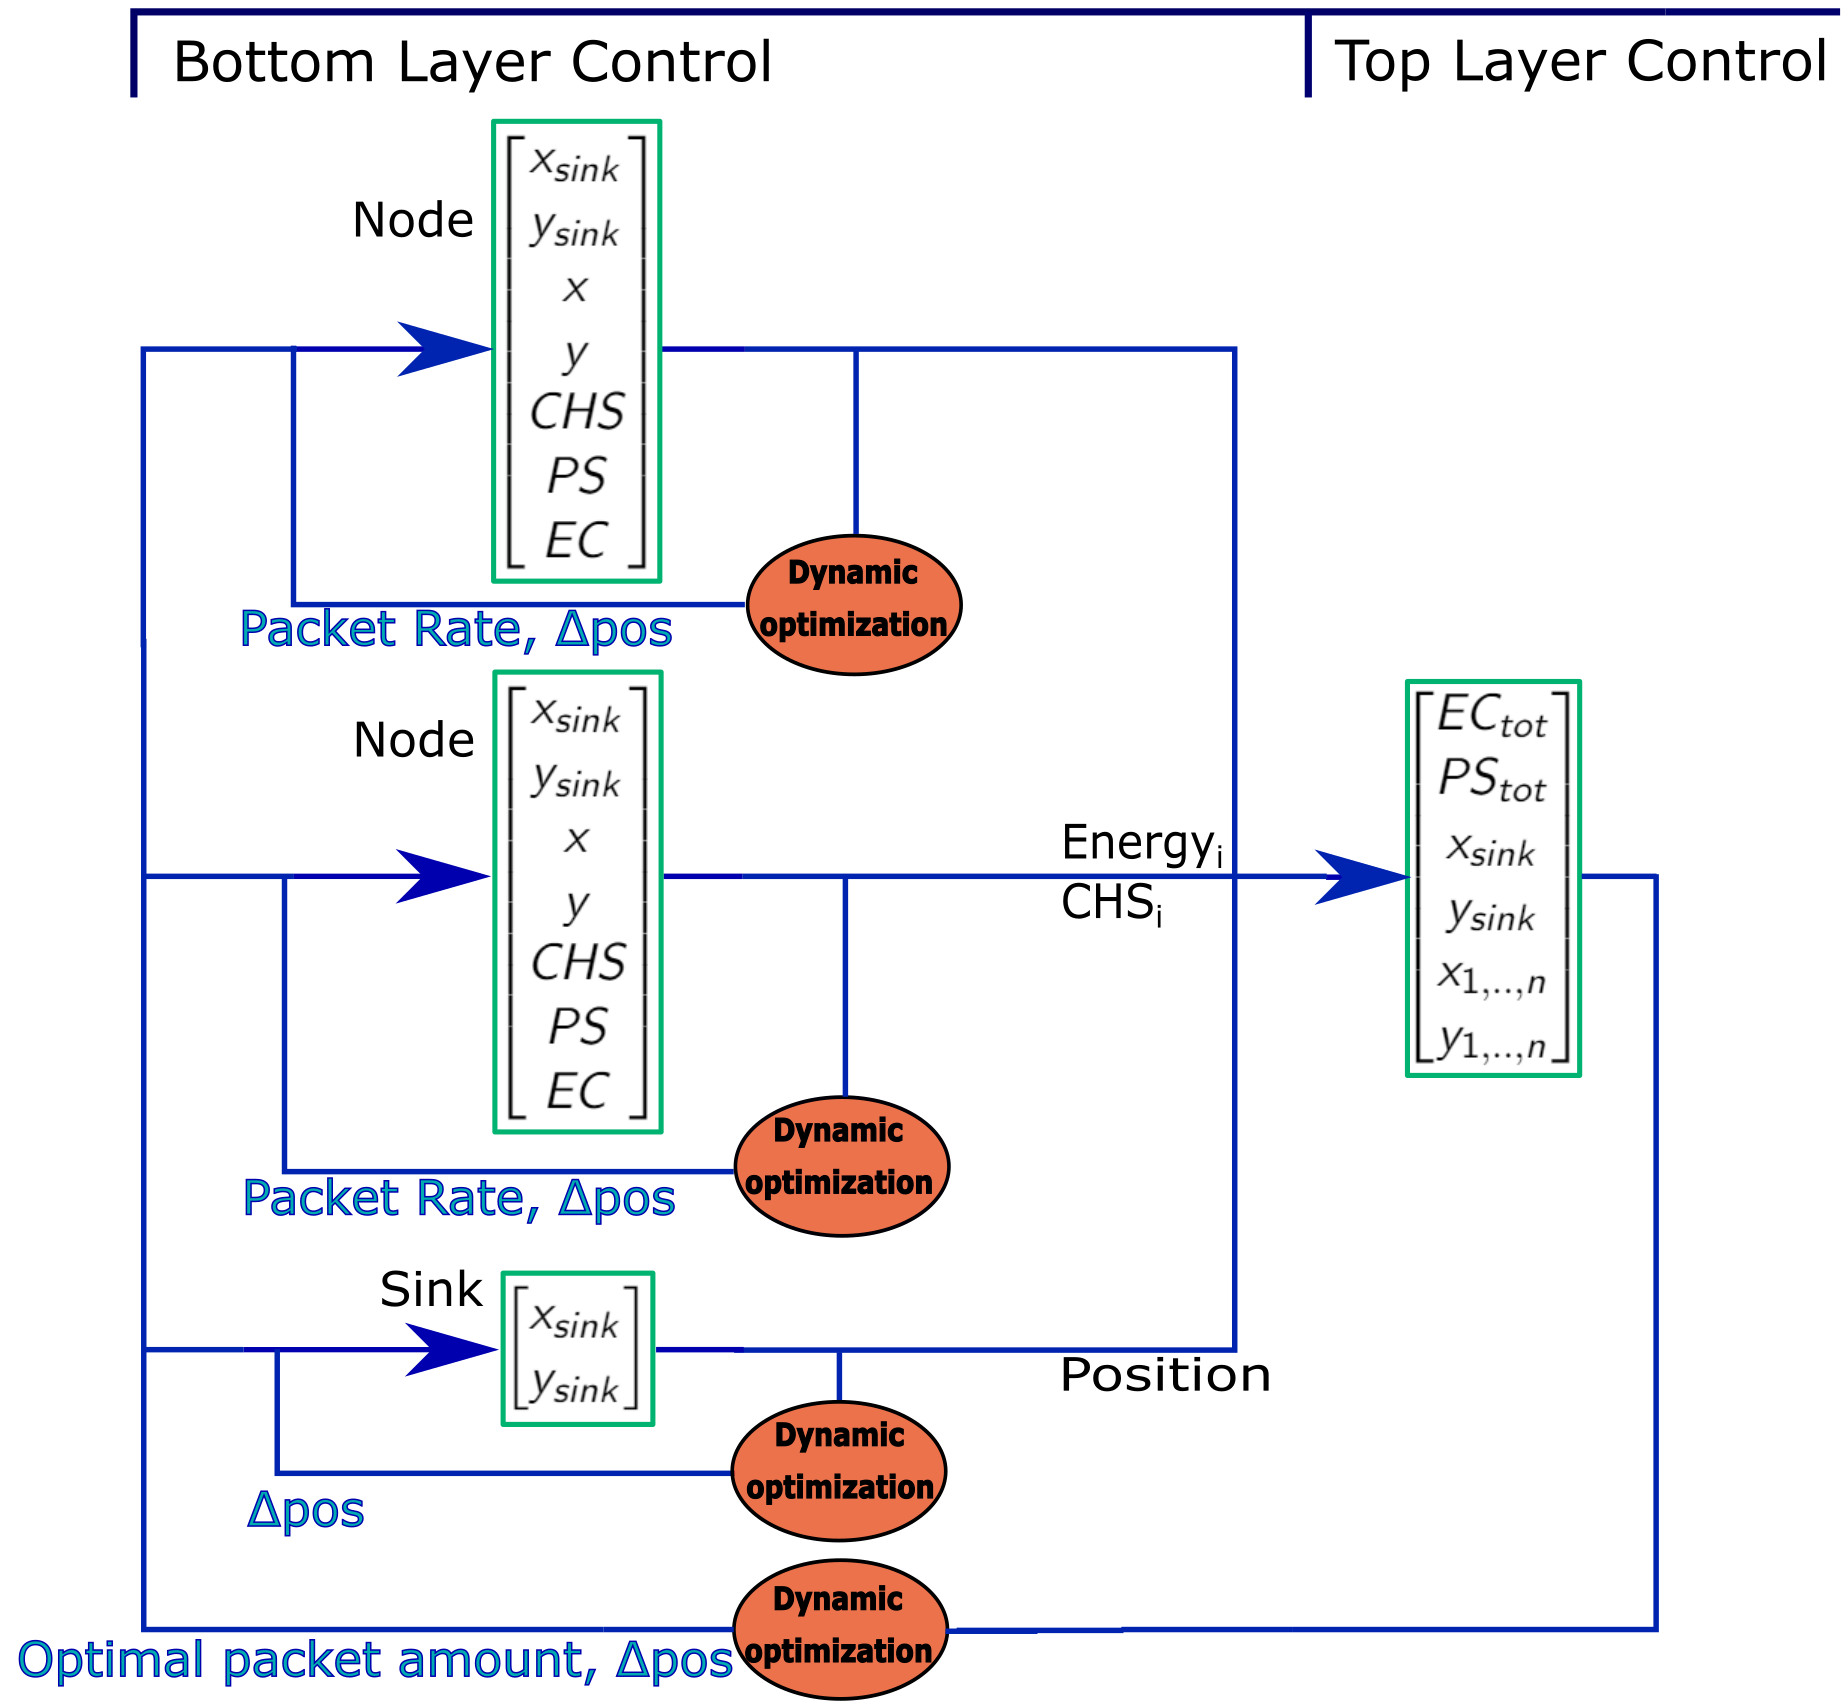
\includegraphics[scale = 0.4]{Images/splitcontrol.png}
    \caption{Architecture for the multi-layer control cooperation.}
    \label{fig:splitctrl}
\end{figure}
\subsection{Upper Layer Control}
\noindent The upper layer control (ULC) aims to solve for an optimal position of the sink as well as an optimal total amount of packets to be sent by each active CH during a transmission round. Since the setup of CHs changes completely as well as in a stochastic manner between every transmission round, planning for control signals beyond the current transmission round was not striven after. Furthermore, by leaving the task of planning for transmission timings to the lower layer control (LLC), this control layer does not take time steps into account. Instead the objective is based on maximizing a quota consisting of packages sent divided by the sum of energy to be spent by the CHs for the current cluster setup. It thus seeks to maximize $bit/J$ for each consecutive round.  \newline

\noindent The optimization goal was defined as
\begin{equation}
    J_{UL}^{*} = maximize\:\frac{\Big( \sum_{i=1}^{N} \delta_{d,i}\Big)}{\Big( \sum_{i=1}^{N} \Psi_{CH,i}\Big)}
\end{equation}
Subject to constraints
\begin{align}
    E_i \geq \Psi_{CH,i}\\
    E_{tot} \geq \sum_{i=1}^{N} \Psi_{CH,i}\\
    0\leq\delta_{d,i}\geq\delta_{d,i,max} \\
    0\leq x_{sink} \leq x_{sink,max} \\
    0\leq y_{sink} \leq y_{sink,max} \\
    \delta_{CH-sink} = \sqrt{(x_{sink}-x_{CH})^{2} + (y_{sink}-y_{CH})^{2}} \label{eq:deltaCHsink}
\end{align}
Here, $\delta_{d,i}$ is the desired amount of packages to be received by the sink from cluster head $i$ for the current round for maximum $bit/J$. Figure \ref{fig:optimizationProbMatlab} shows the modeled constrained solution space for one CH.

\begin{figure}[h]
  \centering
  \subfloat[Solution space, generated in Matlab, of optimizing problem for a single CH with a set amount of connected nodes. The optimization parameters here are the bits desired for a node during a transmission round, the distance between the sink and the CH, and the packets per joule (PPJ) efficiency.]{
  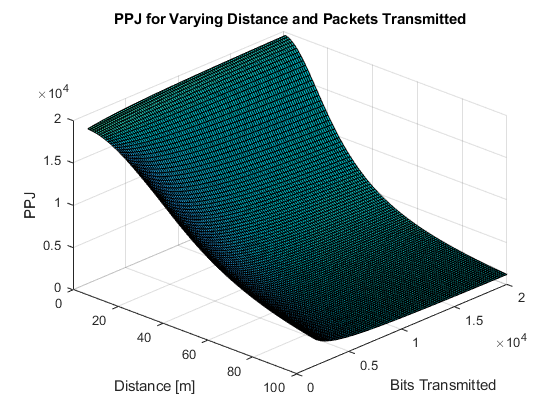
\includegraphics[width=0.45\textwidth]{Images/solutionSpace2ndLayer.png}
  \label{fig:solspace2ndlayer}}
  \hfill
  \subfloat[Solution space for data transmission energy cost for a CH dependent on number of connected child nodes and distance to the sink.]{
  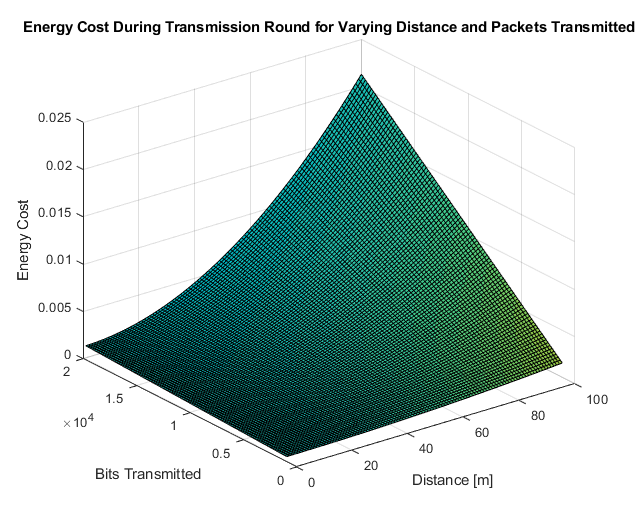
\includegraphics[width=0.45\textwidth]{Images/EnergyCost2ndLayer.png}
  \label{fig:nrjcost2ndLayer}}
  \caption{The solution space for a CH with regards to data transmission energy cost and PPJ.}
  \label{fig:optimizationProbMatlab}
\end{figure}





\subsubsection{Free Nodes}
During almost every clustering period, a number of nodes find themselves closer to the sink than to any nearby CH. These stay connected during the whole transmission round while the sink is moving around. Since these nodes are not being controlled, they were left out of the objective function in order to reduce the computational load further. However, one important observation is that the free nodes under these circumstances are almost always at their closest to their receiver before the sink starts moving. Therefore, all non-CHs were set to send their mandatory package during the first time segment.

\subsubsection*{Practical Method}
The ULC class takes the form of an extension to the environment engine, see Figure \ref{fig:ULCUML}. It works by dynamically building a new model for the current transmission round by polling for which nodes are currently CHs and then stores the state values of the CHs and defines the intermediate equations governing the objectives and constraints. \newline 

\begin{figure}
    \centering
    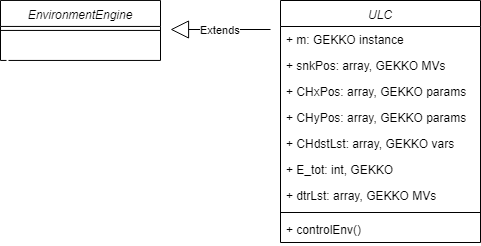
\includegraphics[scale = 0.45]{Images/ULCUML.png}
    \caption{The ULC with its additional functions and attributes as an extension of the Environment Engine class. The GEKKO instance (m) solves for an optimal value for its MVs (each element in dtrLst and snkPos) in order to maximize $bit/J$.}
    \label{fig:ULCUML}
\end{figure}

\noindent The beginning of the implementation process consisted of developing requirements such as:
\begin{itemize}
    \item The optimizer shall produce control inputs that yield an estimated increase of system $bit/J$.
    \item The controller shall posses a fail-safe for any case when the optimizer fails to find a solution.
\end{itemize}

\noindent Initially, the controller was validated and tested for optimizing with respect to a one dimensional distance argument; node positions were simplified to randomized parameter values along $[-50,-49,\hdots,50]$. For each added position, a new GEKKO variable was added for each sink-node distance, $\delta_{CH-sink}$ along with its constraint equation as seen in Equation \ref{eq:deltaCHsink} (two dimensional version). The optimizer was then extended to controlling an additional data transmission rate MV, $dtr$, for each node. Finally, the MV for the position of the sink and the multiple $\delta_{CH-sink}$-variables were split up into their corresponding $x$- and $y$-coordinates. To validate the requirement at each step, the control output of the optimizer and its effect was analyzed and compared with the behaviour of a standard uncontrolled LEACH network. This was done with regards to the summed distance between the sink and all controlled nodes as well as the $bit/J$ ratio.  \newline
 
\noindent A fail-safe was also deployed by implementing a catch for the solver in case it should crash. The catch produces a "safe" control input in the same form as a standard LEACH control system would have. Namely, sink positioned in the middle while each CH is required to send the minimum amount of packages.\newline

\noindent While testing the ULC, every generated sink position was recorded to assess the average distance that the sink would want to travel between clusterings. This was done in order to estimate what sink velocity was needed for average performance. 

(value=33.03 MAY BE PLACED IN RESULTS)

\subsubsection{Product}
Once \verb!controlEnv()! is initialized, the optimizer produces outputs as shown in Figure \ref{fig:ULCoutputs}.

\begin{figure}[h]
  \centering
  \subfloat[ULC sink position output. Blue nodes are CHs and their corresponding numbers are their IDs, green nodes are non-CHs connected to a CH, and yellow nodes are free nodes connected directly connected to the sink.]{
  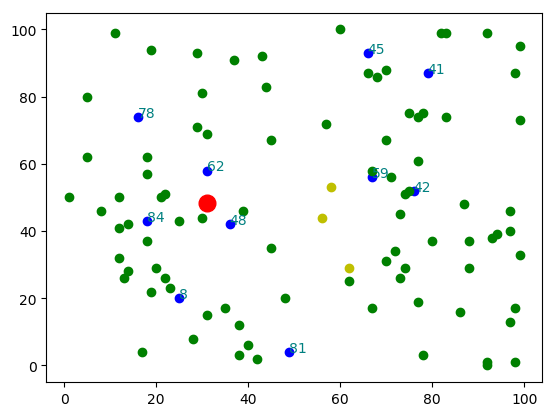
\includegraphics[width=0.45\textwidth]{Images/2ndLayerMap.png}
  \label{fig:ULCmapOutput}}
  \hfill
  \subfloat[ULC $\delta_{d,i}$ output. The desired amount of packages to be sent by each CH with corresponding ID.]{
  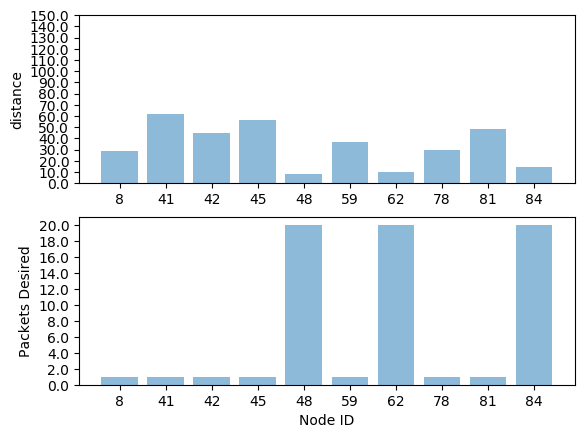
\includegraphics[width=0.45\textwidth]{Images/2ndLayerBar.png}
  \label{fig:ULCbarOutput}}
  \caption{The outputs generated by the ULC. The node ID numbers of a and b are corresponded.}
  \label{fig:ULCoutputs}
\end{figure}


\subsection{Lower Layer Control}
\noindent The LLC aims to optimize for as little energy consumption as possible while still sending the desired amount of packages, $\delta_d$, ordered by the ULC. It does this by controlling the packet rate for each CH during each time segment of the transmission round.\newline  

\noindent The node optimization sub-problem was stated as an objective function consisting of two objectives. Here $\Psi_{node}$ depends on energy consumed by the transmission and $\Phi_{node}$ on the amount of data remaining $\delta_r$ to be sent. The objectives are coupled with weight parameters $Q_{node}$ and $R_{node}$.
\begin{align}
    J_{node}^* = min \: \sum_{n=0}^{K-1} Q\Psi_{node}(k,i,d,b_{tx}) - R\Phi_{node}(K_{deadline},b_{tx}))
\end{align}
Where the objectives were described as
\begin{align}
    \Psi_{node} = E_{Tx}\\
    \Phi{node} = |\delta_r|
\end{align}
The state space model for the node was expressed as
\begin{align}
    E(k+1) = E(k) - (E_{Tx} \\
    \delta_{r}(k+1) = \delta_r(k) - b_{tx}\\
    d(k+1) = v(k)
\end{align}
With state vectors
\begin{align}
    \textbf{x} = [x_{n}, y_{n}, x_{sink}, y_{sink}, \delta_{r}, E]^{T} \\
    \textbf{u} = b_{tx}\\
    \textbf{d} = E_{gen,n}
\end{align}
Subject to constraints for $k\in [0,\hdots,T-1]$
\begin{align}
    0 \leq PA \leq 20 \\
    E \geq [0,\Psi_{node}] \\
\end{align}
The initial states are defined as
\begin{align}
    \delta(0) = \delta_{d}  \\ %delta_desired
    v(0) = v_0
\end{align}

\subsubsection*{Practical Method}
\noindent The following requirements were stated for the LLC:
\begin{itemize}
    \item The optimizer shall produce a control input sequence that result in transmission of as much data as desired by the ULC, or as much as possible if the desired data is an unreachable amount. This data shall be sent before the end of the transmission round.
    \item The controller shall posses a fail-safe for any case when the optimizer fails to find a solution.
\end{itemize}

\noindent The LLC system consists of two cooperating parts, one extension of the Node class and one extension of the Sink class, as shown in Figure \ref{fig:nodeUML}. 

\begin{figure}[h]
  \centering
  \subfloat[Node part of the LLC with  additional functions and attributes as an extension of the Node class. The GEKKO instance (m) solves for an optimal value for its MV (PA during each time segment) in order to minimize the total $\Psi_{node}$.]{
  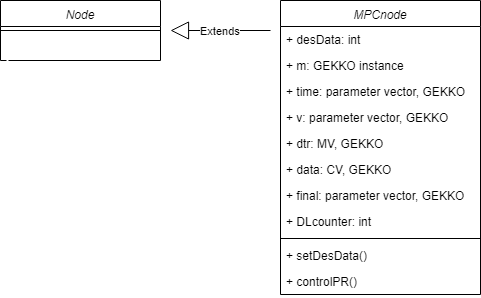
\includegraphics[width=6cm, height=4cm]{Images/nodeUML.png}
  \label{fig:nodeUML}}
  \hfill
  \subfloat[Sink part of the LLC with additional functions and attributes as an extension of the Sink class. MVs are $x$ and $y$ movement.]{
  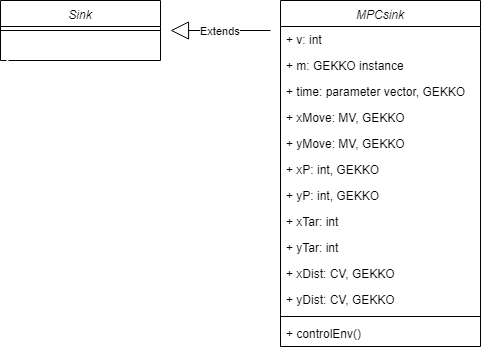
\includegraphics[width=6cm, height=4cm]{Images/sinkUML.png}
  \label{fig:sinkUML}}
  \caption{UML representations of the node and sink extensions.}
  \label{fig:LLCUML}
\end{figure}

\noindent The algorithm starts of by updating the set point of both classes, see Figure \ref{fig:LLCflowchart}. The sink solves for its planned trajectory and stores it in \verb!xP! and \verb!yP!, which can then be polled by any node in order to generate their packet rate control horizon. The trajectory is solved with a fixed horizon length and the endpoint constraint is time-shifted until the current time arrives at the final time constraint ("deadline" in Figure \ref{fig:LLCflowchart}). This is done by coupling the value of $\Psi_{node}$ to a parameter vector \verb!final = [0,...,0,1]! with \verb!length()! equal to the horizon length. The \verb!1! is then shifted as the horizon draws closer to the deadline time constraint. In this case, the final time constraint is always set as the end of the transmission round. A fail-safe was also deployed here with a similar strategy as in the ULC. If no solution is found, the node sends the minimum amount of packages by the end of the transmission round.

\begin{figure}
    \centering
    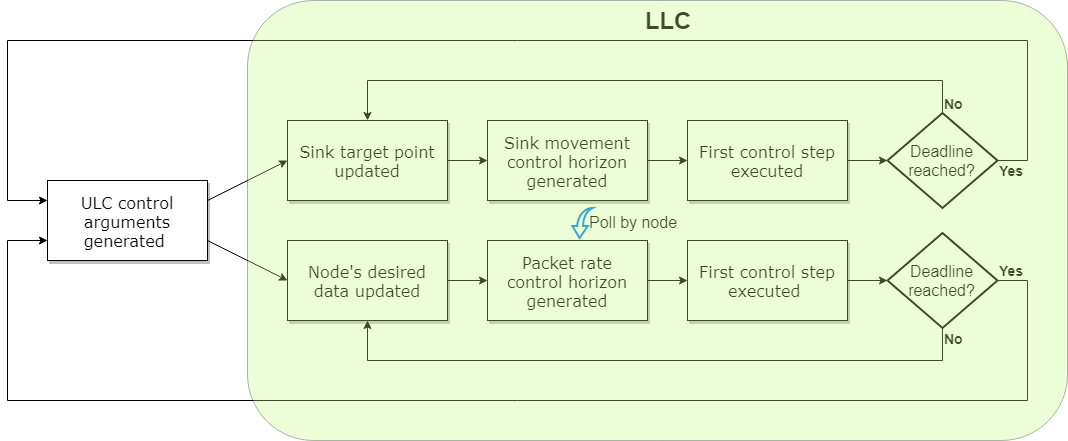
\includegraphics[scale=0.35]{Images/LLCflowchart.png}
    \caption{Flowchart describing the action sequence of the LLC.}
    \label{fig:LLCflowchart}
\end{figure}

\subsubsection{Product}
When \verb!controlPR()! and \verb!produce_MoveVector()! are initialized, the following horizons are generated by the GEKKO modules. See Figure \ref{fig:ULCoutputs}.

\begin{figure}[h]
  \centering
  \subfloat[Control horizon for a node. As shown in the figure, the node plans its transmission for when the sink is at its closest distance (when it passes by).]{
  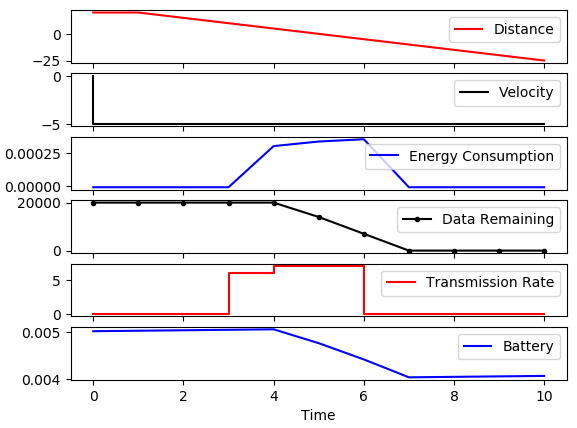
\includegraphics[width=0.45\textwidth]{Images/1stLayerNodePlot.png}
  \label{fig:FirstLayerNode}}
  \hfill
  \subfloat[Control horizon for the sink.]{
  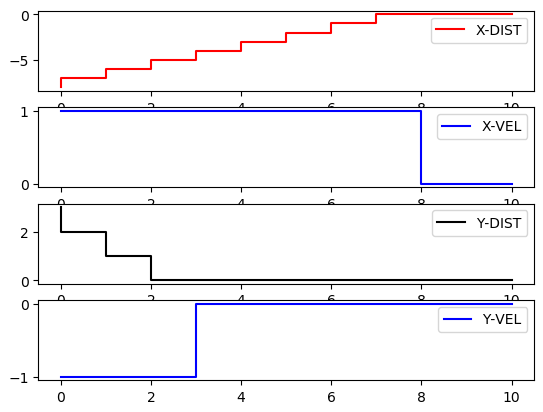
\includegraphics[width=0.45\textwidth]{Images/1stLayerSinkPlot.png}
  \label{fig:FirstLayerSink}}
  \caption{The outputs generated by the LLC. The planned positions of the sink generated by the sink MPC are used by the node MPC in order to plan its transmission timings.}
  \label{fig:LLCoutputs}
\end{figure}

\newpage

\section{RL Design}

\noindent In accordance with the previous discussions on the choice of data driven controller, see Section \ref{sec:ctrlstrategies}, a RL approach was selected. Further, it was decided that the DQN algorithm was the best choice for controlling the mobile sink due to that the WSN environment consisted of a large number of states and actions. The development procedure of the DQN controller was based on the below stated requirements. \newline

\begin{itemize}
    \item The sink/controller shall send as many data packets as possible whilst minimizing the distance to the nodes. 
    \item The amount of states and actions shall be as few as possible to avoid the curse of dimensionality.
    \item The sink shall be movable and the PR of the nodes regulatable.
    \item The controller shall train in the \verb!EnvironmentEngine! simulation environment.
\end{itemize}

\noindent To fulfill the first requirement, the reward was positive for an increase in data packets sent and negative for an increase in distance between the nodes and the sink for the specific case of controlling the sink. The action set $\mathcal{A}$, i.e. the possible actions that the sink could take, was defined as

\begin{equation*}
\begin{multlined}
    \mathcal{A}\:\epsilon\:\{up, down, left, right, diagonal, \\ reduce\:data\:packets\:sent, increase\:data\:packets\:sent\}  
\end{multlined}
\end{equation*}


 \noindent This implies that it was possible for the sink as agent to move right, left, up, down and diagonally with a predetermined step length as well as adjusting the PR of all the nodes. All the states that the agent could be in were determined by a combination of the position of the sink, CH status of all nodes and PR of all nodes. \newline

\noindent Due to the reasoning in Section \ref{sec:softwaretools} regarding the machine learning tools, it was decided to use TensorFlow with Keras running on top of it. The Keras API was deployed to set up the NN and to tune its weights with a built-in optimizer. Based on the mean absolute error of the NN, the optimizer updated the weights such that the loss in Equation \ref{eq:mse} was minimized. Furthermore, the gym library developed by OpenAI was used to setup the WSN in a RL context. \newline

\noindent For controlling the mobile sink with a DQN, the amount of neurons in the input layer of the NN corresponded to the number of states and the amount of neurons in the output layer corresponded to the amount of actions. Thereby the only parameters that needed to be designed were the amount of hidden layers, the amount of neurons in each hidden layer and the learning parameters i.e. the learning rate $\alpha$, discount factor $\gamma$ and the exploration rate $\epsilon$.

% These design choices will be described further in Subsection \ref{sec:RLdesignchoices}.     

\subsection{Design choices}
\label{sec:RLdesignchoices}
In order to design a reliable and fast learned RL controller, several design choices needed to be made. This subsection will declare, describe and motivate the choices that were made during the design of the RL controller.  

\begin{itemize}
    \item \textbf{Learning rate $\alpha$} --- The learning rate shall be in the order of $10^{-3}$, as stated by Thoma \cite{Thoma2017}. If $\alpha$ is too small the learning process will be longer and if $\alpha$ is too large the learning will not converge. Since the time factor is not of priority in this study, the learning rate was chosen to be $10^{-2}$. \newline
    \newline
    \noindent Furthermore, the learning rate was made to adapt to changes in the environment by using a state of the art NN optimizer called Adam-optimizer. A study has found that adapting the learning rate using the Adam-optimizer outperforms a range of other optimizers \cite{kingma2014adam}.

    \item \textbf{Discount factor $\gamma$} --- The discount factor is a variable which determines the amount of future steps the agent will consider when an action is chosen. According to Leissner et al. the discount factor needs to be close to 1 to take actions that are very future oriented \cite{Liessner2019}. The authors also claim that if the discount factor is low the agent will be short sighted and thereby drain its battery immediately. The main challenge was to achieve energy savings at the moment as well as to consider the impacts in the long term. Hence, a decision was made to select the discount factor as $0.8$. 
    
    \item \textbf{Exploration rate $\epsilon$} --- To answer the research question: \textit{"How is the $\epsilon$ value to be selected concerning exploration versus exploitation for the data driven optimal control?"}, both a fix and a decaying exploration rate were implemented twice with varying $\epsilon$-values. The fixed $\epsilon$-values were selected as $0.1$ and $0.15$. The reason for this was that a large $\epsilon$-value would cause the agent to frequently select an deficient action during the late phase of training when it has already built up a relatively good model of the environment. \newline  
    
    \noindent To explore the large number of states and actions of the WSN environment, the initial exploration rate was chosen to be as large as possible for the decaying $\epsilon$ tests, namely $1$. After each action, $\epsilon$ was decayed by multiplying the current exploration rate with a decay factor. The exploration rate was decreased by following the previous procedure until it reached a predefined minimum exploration rate. For the decaying $\epsilon$ tests, the decay factors were set to $0.9995$ \& $0.995$ and the minimum exploration rates were set to $0.05$ \& $0.01$ respectively for the two tests. See Table \ref{tb:epsilonchoice} for a summary of the different exploration rates that were tested. Note that the initial exploration rates were the $\epsilon$-values that were used throughout the entire learning process for the fixed $\epsilon$ tests.
        
    \begin{table}[h!]
        \centering
        \caption{Choices of exploration rate}
        \label{tb:epsilonchoice}
        \begin{tabular}{llcccll}
            \toprule
                     &        &\textbf{Initial $\epsilon$} & \textbf{$\epsilon$ decay factor} & \textbf{$\epsilon$ minimum}\\
            \midrule
         Decaying $\epsilon$  & Test 1 & 1 & 0.9995 & 0.05\\
                     & Test 2 & 1 & 0.995 &  0.01\\ \midrule
         Fix $\epsilon$       & Test 1 & 0.15 & n/a &  n/a\\ 
                     & Test 2 & 0.1 & n/a &  n/a\\
            \bottomrule
        \end{tabular}
    \end{table}

    
    \item \textbf{Reward} --- For the WSN environment a positive reward was given for an increase in amount of data packets sent and a negative reward was given for an increase in distance between the sink and the nodes. The rewards for the two factors were tuned based on multiple trials of various ratios between the two reward factors. Based on constant learning parameters, i.e $\alpha$, $\gamma$ and $\epsilon$ along with the outcome of each trial the rewards were changed such that the desired behaviour was achieved. For instance, if the agent survived a large number of rounds but sent few packets, the reward factor for the amount of data packets sent was increased.
    
    \item \textbf{Amount of hidden layers} --- The accuracy of a NN will increase if the amount of hidden layers are increased until a point when the learning is saturated and the accuracy will start to decrease \cite{he2016deep}. Implementing many hidden layers will also increase the computational load and it is usually enough to use 2 hidden layers according to Heaton \cite{heaton2015artificial}. Due to what was discussed above, 2 hidden layers was chosen for the sink controller. 
    
    \item \textbf{Amount of neurons in hidden layers} --- According to the rule of thumb the amount of neurons in the hidden layers shall be less than double the amount of neurons in the input layer \cite{heaton2015artificial}. The decision was made to select 24 neurons and 48 neurons for the first hidden layer and the second hidden layer respectively.     
\end{itemize}

\noindent Table \ref{tb:RLdesign} below summarizes the choices of the design parameters and Algorithm \ref{alg:dqn} depicts the DQN algorithm in pseudo code. 

\begin{table}[h!]
    \centering
    \caption{RL design parameter choices}
    \label{tb:RLdesign}
    \begin{tabular}{ 
        l % left aligned column
        l % left aligned column
        *{3}{S[table-format=4.0]} % three columns with numeric data       
    }
        \toprule
        \textbf{Parameter} & \textbf{Value}  \\ 
        \midrule
        Learning rate, $\alpha$ & $0.01$ \\
        Discount factor, $\gamma$ & $0.8$ \\
        Optimizer & Adam \\ 
        No. of hidden layers & 2 \\
        No. of neurons in hidden layer 1  & $24$ \\
        No. of neurons in hidden layer 2  & $48$ \\
        \bottomrule
    \end{tabular}
\end{table}


\begin{algorithm}
\caption{DQN Algorithm}\label{alg:dqn}
\begin{algorithmic}[1]
\State Import libraries 
\State Create instance of WSN environment
\State Create and build NN model 
\For{Amount of training episodes}
    \While{At least one node still alive}
        \State Randomize \textit{value} between $0$ and $1$
        \If{\textit{value} <= $\epsilon$}
            \State Select random action 
        \Else 
            \State Predict action with largest Q-value with NN
        \EndIf
        \State Sink in WSN environment implements the action
        \State Observe reward gained \& append info onto memory array
        \State Update weights of NN by randomly sampling from memory array
        \If{\textbf{not} fixed $\epsilon$}
            \State Decay $\epsilon$ by multiplying with the decay rate
        \EndIf{ \textbf{not}}
    \EndWhile
\EndFor
\end{algorithmic}
\end{algorithm}





\begin{comment}
\subsection{Control Method One, Model Based MPC Approach}
\noindent Model predictive control (MPC) is a control method that is based on solving an open loop optimization problem which contains the system model. The controller development was divided into three sequential parts and this subsection will delve deeper into these parts. 

\paragraph{\textit{Defining the Dynamic Features of the Controlled Objective}}
\noindent 
\noindent \newline The equations governing the energy and data aggregation dynamics of each node in the system is derived from \cite{heinzelman2000energy} and are expressed as
\begin{flalign}
    E_{Tz}(k,d) &= E_{elec}k+\epsilon k d^{2} \\
    E_{Rz}(k) &= E_{elec}*k
\end{flalign}
where $k$ is amount of bits, $d$ is the distance between transmitter and receiver, and $E_{Tz}$ and $E_{Rz}$ are energy used for transmission and receiving respective. Here, a CH does both while non-CHs only do transmitting. Each node's $SoC$ is also able to stochastically generate a relatively small amount of energy during each time step. The movement of the sink is simplified by constraining only it's step size, i.e. the movement dynamics themselves are seen as non-existent. 

\paragraph{\textit{Stating the Control Problem}}
\noindent 
\noindent\newline
The progression of the system from one time step to another could be expressed by the discrete state transitions in the form $x(k+1)=f(x(k),u(k))$. The system takes a nonlinear form due to several reasons. One is the probabilistic CH role assignment. Another is the stochastic variation of connected nodes to each CH and the energy generated by each node. One can also observe that the control signal $PA_i$ is coupled with the non-linear state representation $d_i$, which makes the system control affine \cite{PlanningAlgorithms}.\newline

\noindent The states, control inputs, and outputs are described in vector form as respective $x$, $u$, and $y$ are described as follows
\begin{equation}
\label{x_k}
    x =
    \begin{bmatrix}
        x_{sink} \\
        y_{sink} \\
        x_{1,..,N} \\
        y_{1,..,N} \\
        CHS_{1,..,N} \\
        PS_{1,..,N} \\
        EC_{1,..,N} 
    \end{bmatrix}, \:
    u = 
    \begin{bmatrix}
        \Delta x_{sink} \\
        \Delta y_{sink} \\
        \Delta PA_{1,..,N}
    \end{bmatrix}, \:
    y = 
    \begin{bmatrix}
        0 & 0 & 0 & 0 & 0 & 1 & 1
    \end{bmatrix}
\end{equation}
\noindent where $(\Delta x_{sink}, \Delta y_{sink})$ is the change in position of the sink. The position of node $i\in{\{1,...,j\}}$ nodes is assumed to be static. $PS_i$ is the amount of packets sent, $PA_i$ is a control input deciding how many packets to send each control step depending on the distance $d_i$ from each node $i$ to the sink, and $EC_i$ is energy consumed. Here, CH status, $CHS_i \in [0,1]$ is an indicator of whether the node has been chosen to be a CH or not which would decide if control is to be executed with regards to that node. We get a state space representation such that $x(k+1) = Ax + GBu$ and $y=Cx$. However, with an increasing number of nodes the dimension of the state space increases exponentially.
\paragraph{\textit{Choice of Solving Method\newline}}
\hspace{-0.6cm} \noindent To solve the problem of the ever increasing dimensionality, a strategy involving breaking the optimization problem for the entire state-space into minor optimization problems was formed; one for each node and one for the sink. The outputs of these are then summarized in a greater optimization problem which in turn generates the control inputs for the system.
\noindent A cost function $C(x,u)$ dependent on both economic goals was then to be formed with appropriate weighting parameters.

\end{comment}


\chapter{Methodology}
\label{ch:Methodology}
\textit{The following chapter will describe the methodology for the design process as a whole, rationale for design and method choices, type of research, tools and materials used for the research, as well as data collection, validation and analysis.}

\section{Main Design Process}
Firstly, the intended research field was further investigated to get a deeper understanding of the dynamic properties of the controlled objectives. Subsequently, an energy optimization oriented dynamic model was developed and implemented as an interactive controllable environment. Thereafter, the two controllers which followed two different developing principles, namely data driven and model based design were developed, implemented and tested. \newline

\section{Comparison of Control Strategies}
The comparison of the two controllers', as well as the different clustering methods', performance was done as a strictly quantitative study. By conducting model in the loop (MIL) experiments, the performance of the controllers were evaluated based on three indicators. These consisted of the total consumed energy [J], the total amount of data received by sink, and the average energy consumption proportional to data aggregated [bit/J].\newline

\noindent Precautions concerning the validity of the results were taken in order to compare the systems under as equivalent circumstances as possible for the different technical indexes.\newline

\noindent For measuring the efficiency of data aggregated to the sink in relation to energy consumed for each round, identical coordinates for each WSN node was used among the tested systems. The systems were also made to generate an identical set of CHs for each round. The systems were then observed until the first power failure of any node among the test subjects, since the systems will not be fully comparable anymore once this occurs.\newline

\noindent When comparing only the amount of data aggregated to the sink by the controllers, the systems were observed until power failure for all nodes. Identical coordinates for each WSN node were used. However, identical CH role sortings for each consecutive round could not deployed since the systems were to be observed at times where differing amounts of WSN nodes are alive. Therefore, multiple results for each test case were gathered to derive a statistical mean in order to compare the systems.\newline

\noindent The performance of both clustering methods were compared in terms of data packets aggregated to the sink and data packages sent per energy unit. This was done with a stationary sink with identical coordinates for each node as well as identical $p$ values, see \cite{heinzelman2000energy}.\newline

\section{Research Tools and Materials}
The thesis work experiments were executed by conducting simulations in a Python-based test environment, see Appendix \textcolor{red}{[ADD REFERENCE TO APPENDIX]}. Matlab was also used for visualizing and analyzing theoretical behaviour of the LEACH module, as well as the data derived from system test runs.

\section{System Identification and Modeling}
A thorough review of the dynamics of the system and their implementation into the test environment were made initially. Thereafter, verification tests were conducted; values derived from the generated model were compared with the test environment state outputs collected from before and after a discrete time step.

\subsection{Design Decisions}
Requirements engineering was deployed for every design step \cite{6146379}. Functional requirements were specified for each module based on features that had been deemed desirable during the literature review, see Chapter \ref{ch:LitReview}. Each module requirement was connected to test cases which had to be passed in order to advance.


\noindent \textcolor{red}{TODO: Describe what tests has been done and how they were performed} \newline
\textcolor{red}{TODO: What "numbers" were used in the testing, i.e what was the grid size, how many nodes, initial energy etc.}




\chapter{Results}
\textit{In this chapter the results from the simulations and tests of both the MPC controller and the RL controller will be depicted and the performance will be matched against each other.}

\section{BLEACH}

\section{Model Based Controller}

Average computation time per control step for each node at about 0.04s
Average computation time per control step for 2nd layer at about 0.3s


\section{Data Driven Controller}
 This section will present the results from the tests on the data driven controller. The energy consumed, rounds survived and data packets sent will be depicted for all selected explorations rates and compared with LEACH for two different cases. These two cases will be clarified in the following subsections.  

\subsection{Identical CH Generation}
% Explain this test
In the first test with decaying the exploration rates were set to 

\chapter{Discussion and Conclusions}
\textit{The forthcoming chapter presents a discussion based on the results from the testing of the two control methods. Furthermore, conclusions will be drawn from this work and the research questions will be answered.}


\section{BLEACH}
% How did BLEACH perform in comparison to LEACH?

\section{Control Approach}
% Compare the two control approaches together with LEACH based on these three factors
\subsection{Data Packets}
\subsection{Energy Consumption}
\subsection{Data Sent per Energy Unit}

\section{Conclusion}
% Answer RQs here

\chapter{Recommendations and Future Work} 
\textit{In this chapter the future work regarding control of the mobile sink will be discussed. Also, recommendations for improving the WSN environment will be offered. \newline}
\newline
% WSN dynamics
\noindent Currently, the WSN environment consists of a two dimensional grid with an arbitrary amount of nodes and a sink. The energy consumed by a node is solely modelled as a function of the distance \& data packets when data is being sent \& received. This implies that energy losses such as battery leakage and energy consumption due to corrupt data being resended is not modelled. Additionally, the energy consumption and the dynamics of the mobile sink were disregarded. If the WSN model is extended to a 3D space and the aforementioned WSN dynamics are included, it would give a better representation of the physical world. One simulating environment that can handle these dynamics is named OmNet++ \cite{varga2008overview}. \newline
\newline
% Hardware application
\noindent This work has mainly focused on the software and thereby the hardware aspect was not taken into consideration. If this concept of energy management for WSN is to be applied, a further study needs to be conducted on the feasiblity of the algorithms. The study needs to investigate whether the current state of the art processors are capable of handling the computational load of the two algorithms in a timely manner. \newline
\newline
% Choice of parameters (RL)
\noindent The DQN approach of controlling the sink has a limitation in that the agent could only select one action during one time segment. Since the best action could have been a combination of the current available actions, e.g. move sink and send less data packets simultaneously, it would be of interest to analyze the impact of this aspect. Another improvement of the RL approach would be to delve deeper into the design choices of the NN and learning parameters. By selecting more optimal parameters, the learning process could become more effective and thereby shortened. \newline

% MPC
\textcolor{red}{TODO: Write about future work regarding MPC} \newline

\textcolor{red}{Write about the following topics in future work}
\begin{itemize}
\color{red}
    \item (Include the dynamics of the sink)
    \item Make the system handle moving nodes
    \item (Implementation on hardware)
    \item (Extend WSN system to work in 3D)
    \item (More realistic conditions, e.g. resending of packets due to data being corrupted when sending/receiving requires more energy (OMNeT++?))
    \item "Tuning" of the learning parameters, reward and MPC parameters 
    \item ((RL) Controlling several actions at one time step, sink being able of moving in dynamic steps) 
    \item (Energy consumption of sink)
\end{itemize}





\pagebreak
\bibliographystyle{ieeetr}
\bibliography{references}

\appendix
\addappheadtotoc

\chapter{WSN Environment}

The figures below show the WSN environment that was built by the authors. 

\noindent \textcolor{red}{TODO: Put picture of WSN here}




\end{document}
